\documentclass[mscthesis]{usiinfthesis}
\usepackage{lipsum}
\usepackage{listings}
\usepackage{float}
\usepackage{tabularx}

\lstdefinelanguage{algebra}
{morekeywords={import,sort,constructors,observers,transformers,axioms,if,
else,end},
sensitive=false,
morecomment=[l]{//s},
}



\title{Blochchain BAR Gossip} %compulsory
\specialization{Finantial Technology and Computing}%optional
\subtitle{Reliable and clustered gossiping protocol} %optional 
\author{Gianmarco Fraccaroli} %compulsory
\begin{committee}
\advisor{Prof.}{Fernando}{Pedone} %compulsory

\end{committee}
\Day{Yesterday} %compulsory
\Month{September} %compulsory
\Year{2019} %compulsory, put only the year
\place{Lugano} %compulsory

\dedication{To my beloved} %optional
\openepigraph{Someone said \dots}{Someone} %optional

%\makeindex %optional, also comment out \theindex at the end

\begin{document}

\maketitle %generates the titlepage, this is FIXED

\frontmatter %generates the frontmatter, this is FIXED

\begin{abstract}
This is a very abstract abstract. 
\end{abstract}

% \begin{abstract}[Zusammenfassung]
% optional, use only if your external advisor requires it in his/er
%language 
% \\

%\lipsum
%\end{abstract}

\begin{acknowledgements}
\end{acknowledgements}

\tableofcontents 
\listoffigures 
\listoftables %optional

\mainmatter

\chapter{Introduction}
During the last ten years, after the born of Bitcoin, blockchain-based systems became an important building block in several applications, ranging from financial to legal services. As the need for this kind of distributed structured grew, more advanced and sophisticated versions have been built to meet real-world throughput demands. \\
In fact, as the current Bitcoin protocol can handle only seven transactions per second, other protocols like Tendermint or Hyperledger can handle volumes of operations in the order of thousands per second. \\
This is because the latter systems differ in the consensus mechanism, allowing for better performance and higher scalability at the cost of less decentralization. \\
One of the aspects which is typical for most of those systems is the fact that they exchange information through a gossip protocol. Most of the time, this network can be freely joined by anyone, meaning that everyone receives and share updates on the state with other peers. 
As receiving updates reliably and quickly is a key aspect for these kinds of protocols, the P2P network is a crucial aspect as it offers many advantages and disadvantages. \\
Building a faster, safer, and more reliable gossip protocol for blockchains would improve the overall of those systems, making them closer to real-world scenarios needs.


\section{Motivation}
Blockchain systems offer an alternative way to settle an operation between two parties without having to rely on a trusted third party. The most famous and common example is the use of Bitcoin as a method of payments without having to rely on a bank or any other financial service. \\
This is particularly useful because it is possible to decrease the costs associated with the service offered by the mediator and acquire a higher level of trust as the operations can be carried on just by the two (or more) persons involved in the exchange.  \\
As we said before, due to the decentralized nature of these systems, gossip protocols, also called P2P, are heavily employed since they offer a high degree of scalability, fault-tolerance, robustness, fast-spreading and resilience, proprieties which are a perfect match for a decentralized system. \\
Still, these protocols have their disadvantages. First of all, as anyone can join the network without any sort of registration, it is hard to account for their behaviour and punish it. Being not able to punish peers for their incorrect behaviour is even worse in cases where this is done on purpose leading to Sybil or Eclipse attacks (which are going to be discussed later on).\\
So, due to the crucial role of the gossip protocol in a blockchain system, we need to be able to ensure its correctness even in the presence of malicious peers.

\section{Scope}
Gossip protocols used in blockchain-context don't usually take into consideration malicious peer, or if they do, they generally use easy and simplistic countermeasures. 
Since most of the blockchain networks are freely joinable by anyone, malicious peers can't be punished by the system in case of bad behavior as it is always possible for them to change identity and rejoin the system at zero cost.
This thesis aims to find a way to account peers for their behavior, punishing those who either try to gain more benefits at the expense
of other peers or try to slow or even disrupt the system. This goal has to be though in a context where gossip is a crucial aspect of the system, meaning that a slow, inefficient, or expensive protocol would have a significant impact on the overall performance.


\section{Structure of the thesis}
The remaining chapters are going to be structured in the following way. \\
First of all, the next chapter will cover some key concept about blockchains, gossip protocols, and BAR model. \\
The third chapter will then discuss in detail the Blockchain BAR Gossip protocol in all his components, from the model assumption to the different phases. \\
The fourth chapter and fifth chapter will be used to discussed the validity of the implementation of out prototyped simulation and on the experiments derived. \\
Finally, in the last chapter draws the conclusions of this work, discussing some possible future works.

\chapter{Background}
This chapter will outline the concepts and structures related to this thesis in order to better understand the challenges and solutions of the BBAR protocol.

\section{Blockchain}
Blockchain is distributed systems composed of cryptographically linked blocks, where each block store information about the state up to that point in time. Participants in a blockchain network cooperate in order to agree and keep a copy of the common state. This state is often called ledger. \\
Members of the network decide which state is correct by processing information through a common set of rules called consensus. Consensus rules goal is to agree on a common progression of blocks and prevent bad actors from altering it. \\
Blockchain systems are usually divided into three main groups: public blockchains (permissionless), consortium blockchains, and private blockchains (permissioned). \\
The main difference between permissioned and permissionless blockchains is the fact that in the latter, everyone is welcome to be part of the network and take part in the core activities meanwhile the former present a central authority who is in charge of validating, writing information, and selecting who is able to read transactions.  \\
Instead, consortium blockchains, also known as federated blockchain, are semi-public systems controlled by a group of members. They lie in the middle between public and private blockchains. \\
This difference is of key importance for our work as peer identities are unknown in public blockchains and known in private blockchains. Instead, peer identities in federated blockchain are project dependent.

\subsection{Consensus}
As most of the features are common for most blockchain systems, what makes the great majority of them unique is the way they reach consensus. Briefly, it is possible to describe consensus mechanism as the set of rules which make sure that everyone agrees upon which information and state are correct. \\
As we said before, there exist several types of consensus, with the most famous being: Proof of Work, Proof of Stake, Delegated Proof of Stake, and Proof of Authority.
The first one, PoW, is used by Bitcoin and consists of a competition among peers in the network to find a solution to a cryptographic puzzle. These peers are called miners; the "solution" is called hash-puzzle. \\
As more and more peers join the network to find a valid hash-puzzle, the difficulty of the puzzle increase. \\
The second one, PoS, doesn't exploit any computationally hard puzzle but instead gives the possibility to any member of the network to 'stake' an amount of currency to be probabilistically assigned a chance to be the one validating the block. \\
DPoS is similar to PoS but employs a more democratic system to choose the peer who will be validating the next block. The last one is PoA and works in a similar way to PoS. In fact, only a set of peers, called validators, are able, after reaching a supermajority, to add the next block to the chain. Validators are required to stake an amount of currency that will be slashed in case of misbehaviour. Moreover, their identity is public.


\section{Gossip}
Gossip protocols work by periodically exchanging information between members of the network. The exchange works in the following way: first, a peer selects randomly another peer in the system. Later, it contacts the peer and starts to share information with him based on a specific strategy. As peers are chosen randomly, this ensures that there will be a time T in which every peer knowns about every information. \\
These kinds of protocols are usually compared to epidemic diseases as their mathematical proprieties are really similar. One of the main proprieties is the so-called spreading rate, which describes how many hosts get infected as a function of round and the number of infections per host:
$$Y_r = \frac{1}{1 + ne^{-f}r}$$
where $r$ is the round, f is the number a host will infect each round, $Y_r$ is the number of infected hosts in round $r$. Basically, the convergence rate of a gossip protocol is based on how many exchanges he can execute each round and the number of rounds with an increase factor of $e^f$ per round. \\
Benefits of gossip protocols are:
\begin{itemize}
	\item High scalability, as messages need on average $\log(N)$ round to reach every node and node need to send a constant amount of messages independently from the size of the network.
	\item Fault tolerance, since nodes connectivity and irregularities in their behaviour, can be tolerated up to a certain level. Moreover, the same information can be provided by different peers meaning that there is a certain level of redundancy.
	\item High convergence rate, as we have seen above,  peers reach a global state exponentially quickly.
	\item Simplicity, as every node runs the same code.
	\item Resilience, as there are exponentially many routes by which information can flow from its source to its destinations.
\end{itemize}
\newpage
Still, gossip protocols have also his disadvantages:
\begin{itemize}
	\item Fragile with malicious peers, as many attacks can be carried on a gossip protocol that would break the whole system.
	\item Message size limits the scalability of the system, meaning that if information cannot be encoded into a single message, it will require another round of spreading, decreasing the overall scalability.
\end{itemize}
\subsection{Type of gossip protocols}
There exist several kinds of gossip protocol strategies, but most of them are based on the concepts of pull and pull. \\
In push-based strategies, as soon as a node receives a new update, it randomly selects a peer and sends the full payload. This strategy can be further divided into "eager" or "lazy" pull. The lazy version of push-based gossip differs because a node, instead of directly sending the full payload, sends an identifier (such as a hash). The partner will then respond if he wants or not the full payload. \\
Instead, in pull-based strategies, a node randomly selects a peer in the network and ask for recently or available information. Upon receiving that list, they exchange missing information by directly asking the partner for them. \\
Selecting the best strategy is a matter of trade-off: push-based strategies archive a better convergence rate (as they require one less message exchange w.r.t the other strategies) but also produce more redundant data, meaning a higher waste of bandwidth and resources.
There is also the possibility to combine the strategies mentioned above to create more efficient but more complex protocols. \\
One example of such strategy is the eager push and pull, which is characterized by the fact that gossiping is divided into 2 phases: a first one where peers exchange information through a push-based strategy and a second where a pull-based method is used in order to minimize redundant data. \\
Gossip protocols are also characterized by how they manage the membership of the network, as each peer can maintain a full-view or a partial-view of the network and structure of the network, as peers can be organized in tree or circle based shape. % TODO: EXPAND

\subsection{Gossip threats}
Peer in a blockchain network does not usually need to be registrered as no PKI infrastructure exists. This fact is perfect to increase the level of decentralization, but it also introduces no way of punishing a misbehaving peer, as he can easily change his identity.
The most dangerous attacks on this kind of p2p networks are rational attacks, Sybil attack, and Eclipse attacks. \\
The first one includes all those scenarios where a peer acts selfishly the increasing the load of other more altruistic peers. An example is a peer who always asks for updates without sharing anything, minimizing the use of his resources and maximizing his gain. \\
A Sybil attack is a kind of security threat where one person tries to take over the network by creating multiple identities. In a blockchain-context, a malicious actor could create a high number of nodes polluting most of the network's view of other peers. This scenario could lead to a bad situation where most fo peer would not be able to receive or transmit information. \\
Eclipse attacks are a more powerful Sybil attack where an attacker is able to pollute the whole network view of a peer, meaning that the victim cannot understand whether the information he receives is correct or not.
\subsection{Gossip in blockchains}
As of 2019, many blockchains were born, each one providing different services, ranging from financial to juridical and gossip protocol. Most of the time, the p2p network is used to propagate messaging containing blocks or transactions, but there are also examples of blockchain which use gossip to disseminate message for consensus purposes.\\
The most famous and most used blockchain is Bitcoin. In the Bitcoin p2p network, peers maintain a routing table containing the connection information of all the peers they have known about until that time. Every $\Delta$ time $T$, a subset of peers is chosen to start exchange messages using a lazy push-based strategy. Another relevant blockchain is Ethereum, which gossip protocol is pretty similar to Bitcoin's. One relevant fact about Ethereum's p2p protocol is the fact that it has been found vulnerable to an eclipse attack in 2015 and since then a new peer sampling mechanism has been added to remove the issue. \\
Looking at less decentralized blockchain, we have Hyperledger Fabric which divides gossip into push-based and pull-based times. Another one of this kind is Tendermint, which instead follows an eager push-based strategy. Tendermint exploits also gossip to disseminate consensus messages between validators.

\section{BAR model \& BAR Gossip}
Traditionally, fault-tolerance theory admits three different models to describe actor's behaviors, determining how much the system can withstand part of it deviating from the protocol. \\
The first model is the simple fault-tolerance, where the idea is that each actor can either precisely follow the protocol or fail, meaning that the system has to be able to detect and recover from failures. This model is most useful in those scenarios where the system is architecturally decentralized but politically centralized (ex. Google cloud hosting). \\
However, what if the considered system is managed by several organizations or individuals? In this case, the model has to in exchange for the Byzantine fault-tolerance, which states that most of the nodes will follow the protocol, but some of them will deviate either by acting maliciously or because they crash/fail. Byzantine fault-tolerance systems need to survive against a percentage of such deviating members. \\
The last, more realistic and complex model extends the notion of Byzantine fault-tolerance, is called Byzantine Altruistic Rational model an differs from the previous one by adding a simple reasoning: considering a real-life scenario, every actor's behavior in a system is determined by the incentives he gets when following the protocol. Most members of the system will always try to maximize their utility function even if this requires to deviate from the protocol. A simple example are push and pull forms of gossip: as peers are obligated to exchange information in a Tic-For-Tac fashion, they can ask for updates and never sharing them, increasing the load burden on a smaller subset of peers. \\
This is way BAR model assumes three types of actors:
\begin{itemize}
	\item Altruistic: actors who always follow the protocol.
	\item Rationals: actors who follow the protocol if it suits them, and do not follow the protocol if it does not.
	\item Byzantine: actors who only want to disrupt the system.
\end{itemize}
If a system survives under the assumptions of the BAR model, it is said to be incentive-compatible. \\
Looking at the literature, several gossip protocol, assuming the BAR model, have already been studied. One of the most famous is the work done in \{ cite here BAR Gossip\}, which developed the first data streaming application with predictable throughput and low latency. \\
 In BAR Gossip a central tracker distributes updates to a subset of peers, who will then disseminate them with other members of the network in such a way that every peer's action is accountable and provable. As to our knowledge, there is no work on gossip protocols assuming a BAR model in a blockchain-context.
\section{BAR Gossip in details}
Is it worth to explain how BAR Gossip works? Maybe it can lead to easier explanation later.
\section{Problem definition}
Is it worth adding this section to explain which are the problem and challenges of implementing BAR Gossip in a blockchain context?


\chapter{BBAR Gossip}
After having discussed the needed background, we can now move onto describing our BBAR Gossip protocol.\\
 It is important to remember that the primary goal of the protocol is to implement a more reliable p2p network able to withstand or minimize the attack surfaces introduced by p2p protocols. This goal must be persuaded, taking into account that decentralization and convergence rate is a crucial factor in a blockchain network, meaning it could severely impact overall performances.\\
This chapter will start describing the model assumption. It will then move to describe the several kinds of peers included in the network and their relationship. The last three sections will outline the actual protocol with a focus on implementation details and further optimizations.
\section{Model assumptions}
We are making the following assumption about our model:
\begin{itemize}
	\item The p2p network is not built upon any structure.
	\item Every peer in the network adheres to the BAR model.
	\item There exist two kinds of peers: validator and full node.
	\item Validators are block producers and can get punished for misbehaving.
	\item Validators do not know each other. If they need to talk, they do it by gossiping.
	\item Validators are also full nodes and are not recognizable by other peers.
	\item Identities of Validators are known and bound to a Public Key, but their network address is hidden and unknown.
	\item Full nodes keep track of network operations and can generate Proof-of-Misbehavior against malicious peers.
	\item There exist seed-nodes, which a newly joined peer can contact to receive an initial set of peer addresses.
\end{itemize}
Our model assumptions are compatible with most blockchain using PoS as consensus mechanism such as Tendermint.
\section{Cryptographic primitives}
In order to be able to make peers accountable for their actions, we need several kinds of cryptographic primitives: hash function, symmetric cryptography, asymmetric cryptography, and pseudo-random number generators. \\
Hash functions are any function which can be used to map arbitrary length data onto fixed size data. Moreover, we need hashing function with two more additional proprieties:
\begin{itemize}
	\item Pre-image resistance
	\item Second-image resistance
	\item Collision resistance
\end{itemize}
The hashing function chosen in our implementation is SHA256, but other good candidates are SHA3 or BLAKE2. \\
Symmetric encryption is an encryption mechanism that uses the same key to encrypt and decrypt some data. It is composed of an encryption algorithm, a decryption algorithm, the plain-text, the cipher-text, and a secret key. The encryption algorithm takes as parameters the plain-text and secret key and outputs the -cipher-text. The decryption algorithm takes as parameters the cipher-text and secret key and outputs the plain-text. The symmetric encryption algorithm chosen in our implementation is AES256, but Salsa20 or ChaCha are also good candidates. \\
Asymmetric encryption uses two key, one called private and one public, to either encrypt/decrypt or perform digital signatures. Digital signatures are a mathematical technique to validate the authenticity and integrity of a message and are usually used to acknowledge the consent of the signer.  \\
Our implementation uses Elliptic Curve cryptography.
Pseudo-random number generators are algorithms that deterministically generates a sequence of numbers whose properties approximate the properties of sequences of random numbers. PRNGs cannot be considered really random as their output is totally determined by an initial value called seed. Our implementation follows the Mersenne Twister PRNG, but the XORShift PNRG family is also a good candidate.
\section{Type of peers}
BBAR Gossip introduces two new different node types in the network along with the standard validator, full and seed node. It also modifies the default behaviour of seed node. \\
The new nodes are called bootstrap and entry nodes. Each node has a particular role in the network. \\
\begin{itemize}
	\item Bootstrap nodes are the main difference with traditional gossips. Its primary purpose is to register and keep track of new peers, remove malicious peer, and coordinate the exchange of messages. Each Bootstrap node identity is tied to a corresponding validator's identity as they can be made accountable for their actions and, in case of misbehaviour, be slashed.
	\item Entry nodes are an additional component of every bootstrap node. They act as reverse proxies to keep the network identity (IP address) of the bootstrap node hidden to avoid DDoS attacks.
	\item Full nodes are simple peers in the network who want to exchange messages with other peers to sync their state. They have different behaviour as they agree to the BAR model.
	\item Seeds node keep track of bootstrap node's addresses as new peers need to be able to contact a bootstrap node to start interacting with the network.
\end{itemize}

\section{Protocol description}
We have divided the protocol into three phases, which a peer has to follow to start exchanging messages and sync his state. 
\subsection{Epoch concept}
A cardinal concept and crucial building block of the protocol is the notion of Epoch.  \\
An epoch is a $\Delta$ $T$ time used to divide time and synchronize peers, and each Bootstrap node decides how long an epoch last. Epochs have to be a monotonically increasing sequence of numbers and must not overlap.
\subsection{Registraton phase}
We have divided the protocol into three phases, which a peer has to follow to start exchanging messages and sync his state. 

\begin{figure}[h]
  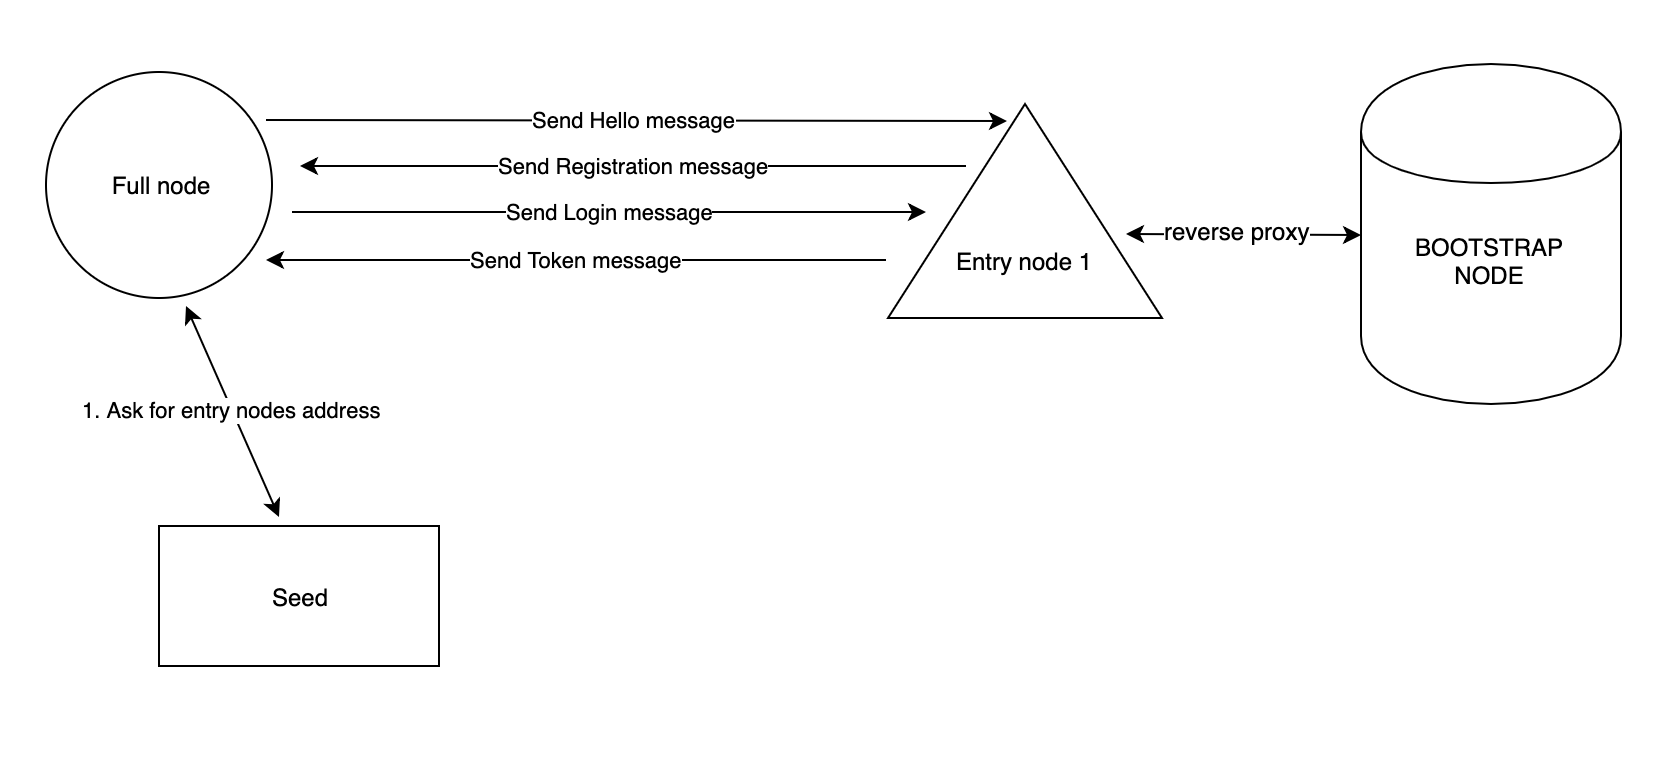
\includegraphics[width=\linewidth]{images/register-phase.png}
  \caption{Register phase chart}
  \label{fig:register-flow}
\end{figure}

The first thing a peer has to do to be included in a network is to contact a seed node to receive some bootstrap's entry points addresses. From the list of addresses, the peer will randomly contact a subset of them and start the following message exchange.
\begin{itemize}
	\item Peer sends a HELLO message[\ref{tab:hello-message}] to the entry node/s, with his public-key and network address.
	\item Entry node/s contact the Bootstrap node and send back a REGISTRATION message[\ref{tab:register-message}] , which includes a Hashcash-style puzzle and the corresponding difficulty.
	\item As soon as the peer finds a solution for the crypto-puzzle, it sends to the entry node/s a LOGIN message[\ref{tab:login-message}], including the solution.
	\item The entry node/s checks the validity of the solution. If the solution is valid, sends back a TOKEN message and includes the peer information in the next epoch. Together with a TOKEN message, a VIEW[\ref{tab:view-message}] message is also sent.
\end{itemize}
  
Each bootstrap node can choose the difficulty of the desired solution, meaning that they can control how many registrations they get on average in the next $T$ epochs.\\
In the last step, after checking that the solution is valid, the entry nodes returns a TOKEN message. The TOKEN message contains a digital signature over the hash of the string generated as the concatenation of the crypto-puzzle, the corresponding solution, and epoch. It is possible for everyone, using this format, to check the validity of the Hashcash solution, (to avoid collusion between the bootstrap node and a peer) and bind the token to a specific epoch. Moreover, the TOKEN message, includes a field called Key, which stores 16 random bytes which will be used later in the protocol. \\
Still in the last step, the entry nodes sends also a VIEW message which contains a list of all the registered peers with their informations and the next epoch 
time. \\
When the next epoch start, every peer in the network has to send back their token to the corresponding Bootstrap node. If the Bootstrap node does not have any PoM against that peer, it will send back a new TOKEN and VIEW message.

\begin{table}[H]
\centering
\resizebox{\textwidth}{!}{%
\begin{tabular}{|l|l|l|}
\hline
           & \textbf{Size}            & \textbf{Description}                                            \\ \hline
\textbf{Host}       & variable length & Network address of the peer                            \\ \hline
\textbf{Port}       & 4 byte          & Network port of the peer                               \\ \hline
\textbf{Public Key} & 33 byte         & Public key encoded as the x coordinate and oddness bit \\ \hline
\end{tabular}
}
\caption{Login message description}
\label{tab:hello-message}
\end{table}

\begin{table}[H]
\centering
\resizebox{\textwidth}{!}{
\begin{tabular}{|l|l|l|}
\hline
           & \textbf{Size}     & \textbf{Description}                                                  \\ \hline
\textbf{Difficulty} & 4 bytes  & Integer describing the difficulty of the solution            \\ \hline
\textbf{Puzzle}     & 49 bytes & Concatenation of the encoded public-key plus a 16 byte nonce \\ \hline
\end{tabular}
}
\caption{Register message description}
\label{tab:register-message}
\end{table}

\begin{table}[H]
\centering
\resizebox{\textwidth}{!}{
\begin{tabular}{|l|l|l|}
\hline
       & \textbf{Size}            & \textbf{Description}                                                  \\ \hline
\textbf{Puzzle} & 49 bytes        & Concatenation of the encoded public-key plus a 16 byte nonce \\ \hline
\textbf{Proof}  & Variable length & The solution to the crypto-puzzle                            \\ \hline
\end{tabular}
}
\caption{Login message description}
\label{tab:login-message}
\end{table}


\begin{table}[H]
\centering
\resizebox{\textwidth}{!}{
\begin{tabular}{|l|l|l|}
\hline
                & \textbf{Size}         & \textbf{Description}                                         \\ \hline
\textbf{Puzzle} & 49 bytes              & Concatenation of the encoded public-key plus a 16 byte nonce \\ \hline
\textbf{Proof}  & Variable length       & The solution to the crypto-puzzle                            \\ \hline
\textbf{Token}  & 71 bytes (on average) & The BN digital signature used as token                       \\ \hline
\textbf{Epoch}  & 4 bytes               & The integer describing the current epoch                     \\ \hline
\textbf{Key}    & 16 bytes              & Random data used as encryption key                           \\ \hline
\end{tabular}
}
\caption{Token message description}
\label{tab:token-message}
\end{table}

\begin{table}[H]
\centering
\resizebox{\textwidth}{!}{
\begin{tabular}{|l|l|l|}
\hline
                    & \textbf{Size}   & \textbf{Description}                                        \\ \hline
\textbf{Peer List}  & Variable length & List of peer and their corresponding PK and network address \\ \hline
\textbf{Epoch}      & 4 byte          & Integer describing the epoch                                \\ \hline
\textbf{Next epoch} & 4 byte          & Unix timestamp of the next epoch time                       \\ \hline
\end{tabular}
}
\caption{View message description}
\label{tab:view-message}
\end{table}



\subsection{Peer selection phase}
As soon a the registration phase is over, a peer should have received a valid token from the TOKEN message and a list of peers he can contact from the VIEW message. \\
Instead of randomly selecting a peer in the peer list, the selection is computed using a PNRG seeded with the token received. The output of the PNRG modulus the size of the peer list will generate the index of the selected partner in the list. \\ If the index number is the peer itself, it generates another random number using the same PRNG, until a valid one comes out.
Using this mechanism, we can make peers accountable for peer-selection and create PoMs in case of misbehaviour. 

\subsection{Exchange phase}
The last phase, called Exchange phase, is heavily inspired by BAR Gossip and exploits a sequence of messages to maintain peers accountable for every decision they make.

\begin{figure}[H]
\centering
  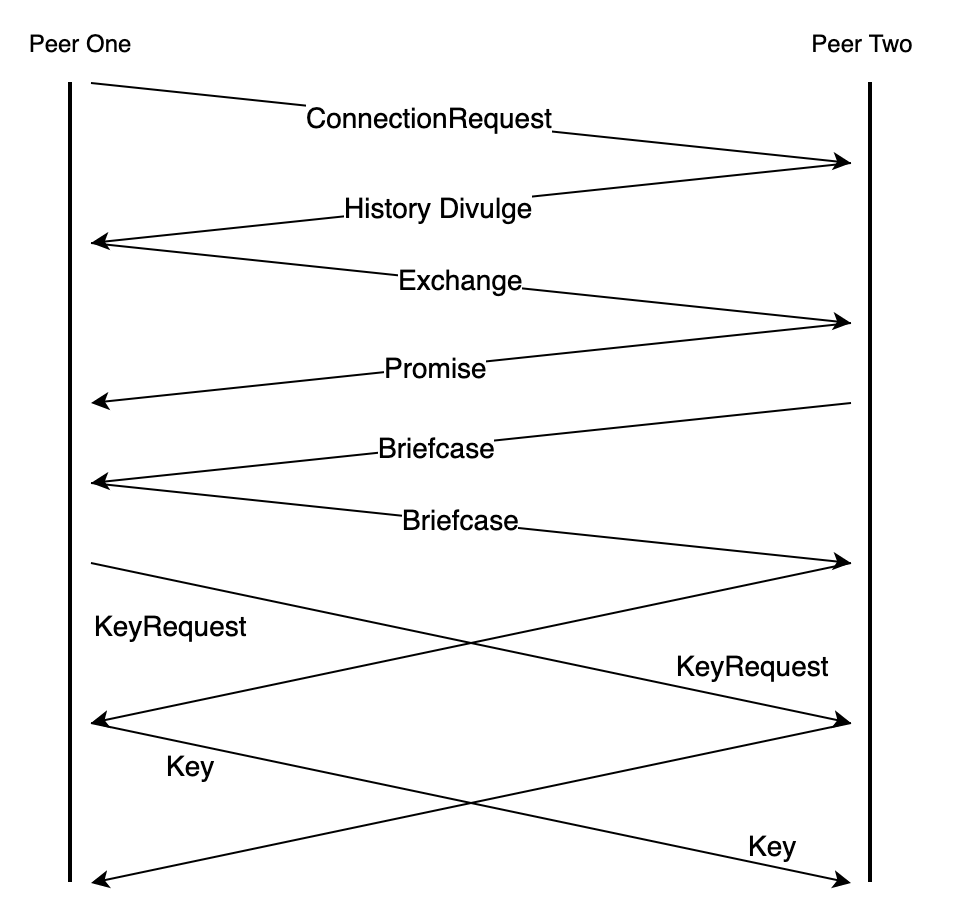
\includegraphics[width=12cm]{images/exchange-phase.png}
  \caption{Exchange phase flow}
  \label{fig:exchange-phase}
\end{figure}

As soon as a peer determined who has to contact, the protocol follows these steps:
As soon as a peer determined who has to contact, the protocol follows these steps:
\begin{itemize}
	\item A CONNECTIONREQUEST[\ref{tab:connectionrequest-bar-message}] message is sent to the selected partner.
	\item After validating the connection, the partner sends back a HISTORYDIVULGE[\ref{tab:historydivulge-bar-message}] message, informing the peer that he has accepted his request and giving him the details about his mempool/state as a list of hash identifiers.
	\item On receiving the HISTORYDIVULGE message, the peer computes the set difference with his mempool/state. Based on those results, it decided if his best choice is a BAR or OPT exchange and sends to his partner an EXCHANGE[\ref{tab:exchange-bar-message}] message containing a list of updates he wants, he will give back and the exchange type to perform.
	\item The partner checks if the exchange is valid (it will be explained later what it means), and sends back a PROMISE[\ref{tab:promise-bar-message}] message, which affirms the fact that he accepted the exchange, and a BRIEFCASE message, which contains the updates encrypted.
	\item Upon receiving a valid PROMISED message, the peer also sends to his partner a BRIEFCASE[\ref{tab:briefcase-bar-message}] message.
	\item Upon receiving a BRIEFCASE message, both peers will start sending a KEYREQUEST[\ref{tab:keyrequest-bar-message}] message to the partner, until either the epoch finish or until a KEY message arrives.
	\item The KEY[\ref{tab:key-bar-message}] message includes the secret to open the corresponding briefcase, containing the requested updates.
\end{itemize}

First of all, each message sent during this phase contains a header containing the token plus relative information to verify his validity and a hash of the previous message, so that it is possible to rebuild the message history. \\
A crucial aspect of the protocol, which is heavily inspired by BARGOSSIP  are the two types of exchanges available: BAL or OPT. A BAL exchange is characterized by the fact each member of the trade promised to exchange the same number of updates, in a TicForTat fashion. As this is not always possible, OPT provided a safe-net mechanism for peers who do not have something to exchange, and they rely on the altruism of other peers. In fact, a peer A who starts an OPT exchange, promises to the other 0 or more updates and asks the partner to send back either the same number of updates as him or more. Moreover, the number of updates exchange during each trade is bounded both for BAL and OPT, as this increase the possibility for a peer to start a BAL exchange. \\
As we want to incentivize the more fair BAL exchange, partner B will add a percentage of random data to the BRIEFCASE message.  \\
A fundamental difference with BAR Gossip is the fact that the peer sending the CONNECTIONREQUEST message, is the one choosing the type of exchange.  \\
The Briefcase message is encrypted using a symmetric encryption algorithm where the secret key is received by the Bootstrap node in the TOKEN message. \\
As in BAR Gossip, all messages are sent through TCP connection expect the KEYREQUEST and KEY message.

\begin{table}[H]
\centering
\resizebox{\textwidth}{!}{
\begin{tabular}{|l|l|l|}
\hline
                            & \textbf{Size}         & \textbf{Description}                                        \\ \hline
\textbf{Puzzle}             & 49 bytes              & List of peer and their corresponding PK and network address \\ \hline
\textbf{Solution}           & Variable length       & Integer describing the epoch                                \\ \hline
\textbf{Epoch}              & 4 bytes               & Unix timestamp of the next epoch time                       \\ \hline
\textbf{Token}              & 71 bytes (on average) & The BN digital signature token                              \\ \hline
\textbf{Prev. Message Hash} & 32 bytes              & The hash of the previous message                            \\ \hline
\end{tabular}
}
\caption{Header description}
\label{tab:header-bar-message}
\end{table}


\begin{table}[H]
\centering
\resizebox{\textwidth}{!}{
\begin{tabular}{|l|l|l|}
\hline
                & \textbf{Size} & \textbf{Description}                                               \\ \hline
\textbf{Header} & Variable size & The header of the message used to verify the peer request validity \\ \hline
\end{tabular}
}
\caption{ConnectionRequest message description}
\label{tab:connectionrequest-bar-message}
\end{table}

\begin{table}[H]
\centering
\resizebox{\textwidth}{!}{
\begin{tabular}{|l|l|l|}
\hline
                    & \textbf{Size}              & \textbf{Description}                                               \\ \hline
\textbf{Header}     & Variable size              & The header of the message used to verify the peer request validity \\ \hline
\textbf{Update ids} & Number of updates * 20 bytes & The list containing the identifiers of the updates                     \\ \hline
\end{tabular}
}
\caption{HistoryDivulge message description}
\label{tab:historydivulge-bar-message}
\end{table}

\begin{table}[H]
\centering
\resizebox{\textwidth}{!}{
\begin{tabular}{|l|l|l|}
\hline
                  & \textbf{Size} & \textbf{Description}                                               \\ \hline
\textbf{Header}   & Variable size & The header of the message used to verify the peer request validity \\ \hline
\textbf{Needed}   & Variable size & Identifiers of updates the peer needs                              \\ \hline
\textbf{Promised} & Variable size & Identifiers of updates the peer will trade                         \\ \hline
\textbf{Type}     & 1 byte        & The type of exchange: BAL, OPT or ABORT.                           \\ \hline
\end{tabular}
}
\caption{Exchange message description}
\label{tab:exchange-bar-message}
\end{table}

\begin{table}[H]
\centering
\resizebox{\textwidth}{!}{
\begin{tabular}{|l|l|l|}
\hline
                  & \textbf{Size} & \textbf{Description}                                               \\ \hline
\textbf{Header}   & Variable size & The header of the message used to verify the peer request validity \\ \hline
\textbf{Needed}   & Variable size & Identifiers of updates the peer needs                              \\ \hline
\textbf{Promised} & Variable size & Identifiers of updates the peer will trade                         \\ \hline
\textbf{Type}     & 1 byte        & The type of exchange: BAL, OPT or ABORT.                           \\ \hline
\end{tabular}
}
\caption{Promise message description}
\label{tab:promise-bar-message}
\end{table}


\begin{table}[H]
\centering
\resizebox{\textwidth}{!}{
\begin{tabular}{|l|l|l|}
\hline
                   & \textbf{Size} & \textbf{Description}                                               \\ \hline
\textbf{Header}    & Variable size & The header of the message used to verify the peer request validity \\ \hline
\textbf{Briefcase} & Variable size & The encrypted updates                                              \\ \hline
\end{tabular}
}
\caption{Briefcase message description}
\label{tab:briefcase-bar-message}
\end{table}

\begin{table}[H]
\centering
\resizebox{\textwidth}{!}{
\begin{tabular}{|l|l|l|}
\hline
                & \textbf{Size} & \textbf{Description}                                               \\ \hline
\textbf{Header} & Variable size & The header of the message used to verify the peer request validity \\ \hline
\end{tabular}
}
\caption{Key Request message description}
\label{tab:keyrequest-bar-message}
\end{table}

\begin{table}[H]
\centering
\resizebox{\textwidth}{!}{
\begin{tabular}{|l|l|l|}
\hline
                & \textbf{Size} & \textbf{Description}                                               \\ \hline
\textbf{Header} & Variable size & The header of the message used to verify the peer request validity \\ \hline
\textbf{Key}    & 16 bytes      & The secret key used to encrypt the briefcase                       \\ \hline
\end{tabular}
}
\caption{Key message description}
\label{tab:key-bar-message}
\end{table}

\section{Details}
\subsection{Proof-of-Misbehavior}
The idea behind PoMs is to have a mechanism to prove that a member of the network tried to deviate from the protocol. In our protocol (as well as in BAR gossip) this is accomplished through the use of cryptography: digital signatures and hash functions are combined to keep each peer accountable.\\
 As soon as a peer misbehaves, the partner can use generate a PoM and send it to the corresponding Bootstrap node, who will schedule an eviction in the next epoch.

\subsection{Shuffle peer list each epoch}
A Bootstrap node could collude with a peer to particularly craft the order peer list in such a way that a peer always contacts the same subset of peers. Due to this issue, the peer list has to be shuffled in a random but verifiable way.  An option which we have used in our implementation to accomplish this task is the following:
\begin{itemize}
	\item Sort the peer list by X coordinate of the public-key.
	\item Seed a PNRG with a public seed (i.e., the current epoch) and generate a sequence of unique numbers from 0 to the size of the list.
	\item Shuffle the peer list according to the generated sequence (i.e., first peer in the sorted list goes to the position specified by the first number in the sequence).
\end{itemize}

\subsection{Multiple BN registration per peer}
An important factor for this protocol is that peers need to be registered with multiple Bootstrap nodes. This is because there has to be at least a path which links all the bootstrap node networks into a single one. Otherwise, peers would be able to exchange only the information inside a single bootstrap network which is only a subset of the whole network. \\ 
Obviously, this comes with a trade-off: the more registration a peer has, the more trades he has to do meaning that he will use more bandwidth and resources.

\subsection{Fair exchange problem}
The reason why a Bootstrap node has to give the secret key for encrypting the briefcase together with the token is that a malicious peer could create some fake updates identifiers to perform a BAL exchange, wait for the partner KEY message and then fake a crash or timeout. Using this strategy, one of the peers receives the updates; meanwhile, the other would not be able to decrypt the BRIEFCASE, which contains garbage data. This problem can be reduced to the fair exchange problem, which is actually impossible to solve without a trusted third party. In our case, the BN node acts as a TTP. If a peer does not receive the KEY message, he can send an MPoM (Maybe-Proof-of-Misbehavior) with the encrypted briefcase. The bootstrap node will decrypt the BRIEFCASE message, check the validity of the updates, and if the updates are legit, send back the key to the peer. Otherwise, it will ban the peer's partner.

\subsection{PoM rewards}
As sending PoM is resource expensive for peers, we need to incentivize this behavior. A possible solution is the following: since bootstrap nodes are linked to Validators which are block producers, we can incentivize this behavior by giving priority of receiving the new blocks to those peers that send valid PoMs or MPoMs.

\section{Optimizations}
There are several ways to improve the performance of the protocol, but the ones with the most gains are the following two.

\subsection{History exchange}
One of the most resource-consuming messages is the HISTORYDIVULGE, as the partner has to provide a list containing a list of hash identifiers. This scale linearly with the number of updates. \\
The more straightforward way to decrease the size of the list would be to encoded the identifiers with a smaller format and to reduce the number of identifiers. This is archivable by:
\begin{itemize}
	\item Using a hash function with a smaller output such as RIPEMD-160.
	\item Heuristically chose a subset of updates
\end{itemize}
A more sophisticated way to accomplish this task is to encode the updates into a more efficient data structure such as an Inverse Bloom Lookup Table or a Set Sketch. \\
Those kind of data structure are very efficient for set reconciliation tasks as they are able to encode data (in our case the identifiers) in a bloom filter fashion but with the added features that it is possible to recover the whole set of encoded data, and it is possible to perform the subtraction between two of them.

\subsection{Message header}
The message header takes a non-trivial amount of bytes in each message. It is possible for each peer to send just the first message with the full header.\\ Meanwhile, the following messages could contain just a hash of it.

\chapter{Evaluation}
\section{BBAR vs BAR}
I am not sure I will be able to plot the necessary data. Can i just explain the difference and similarity with BAR gossip?
\section{Simulation vs Prototype}
In order to evaluate our protocol we decided to implement both a prototype, with all the features described in the previous chapter, and a simulator, which is more scalable and easier to manage. \\
We setup the prototype and simulator with the same parameters: 

\begin{table}[H]
\centering
\resizebox{\textwidth}{!}{%
\begin{tabular}{|l|l|l|}
\hline
                                 & \textbf{Value} & \textbf{Description}                                                  \\ \hline
\textbf{Bootstrap nodes}         & 3              & The number of BNs in the simulation                                   \\ \hline
\textbf{Full nodes}              & 25            & Total number of FN in the simulation. They are ALTRUISTIC by default. \\ \hline
\textbf{Rational nodes}          & 10       & Percentage of rational nodes                                          \\ \hline
\textbf{Byzantine nodes}         & 5       & Percentage of byzantine nodes                                         \\ \hline
\textbf{Epochs}                  & 40            & Number of epochs                                                      \\ \hline
\textbf{PoW Difficulty}          & 3              & Difficulty expressed as number of epochs                              \\ \hline
\textbf{Byzantine level}         & 0.3            & Probability for a byzantine node to act byzantine during an exchange  \\ \hline
\textbf{Mempool size}            & 20, 0         & Mean and standard deviation of peer's mempool size                    \\ \hline
\textbf{Number of subscriptions} & 2       & Number of registration per peer                                       \\ \hline
\textbf{Max BAL exchange}        & 8             & Maximum number of updates per BAL exchange                            \\ \hline
\textbf{Max OPT exchange}        & 15             & Maximum number of updates per OPT exchange                            \\ \hline
\end{tabular}%
}
\caption{Simulation parameters description}
\label{tab:simulation-paramters}
\end{table}
 
Due to some limitation in the prototype implementation and as most of the actions taken are based on a random coin flip, we are not able to run two identically models even if the parameters are the same.

\begin{figure}[H]
   \begin{minipage}{0.49\textwidth}
     \centering
     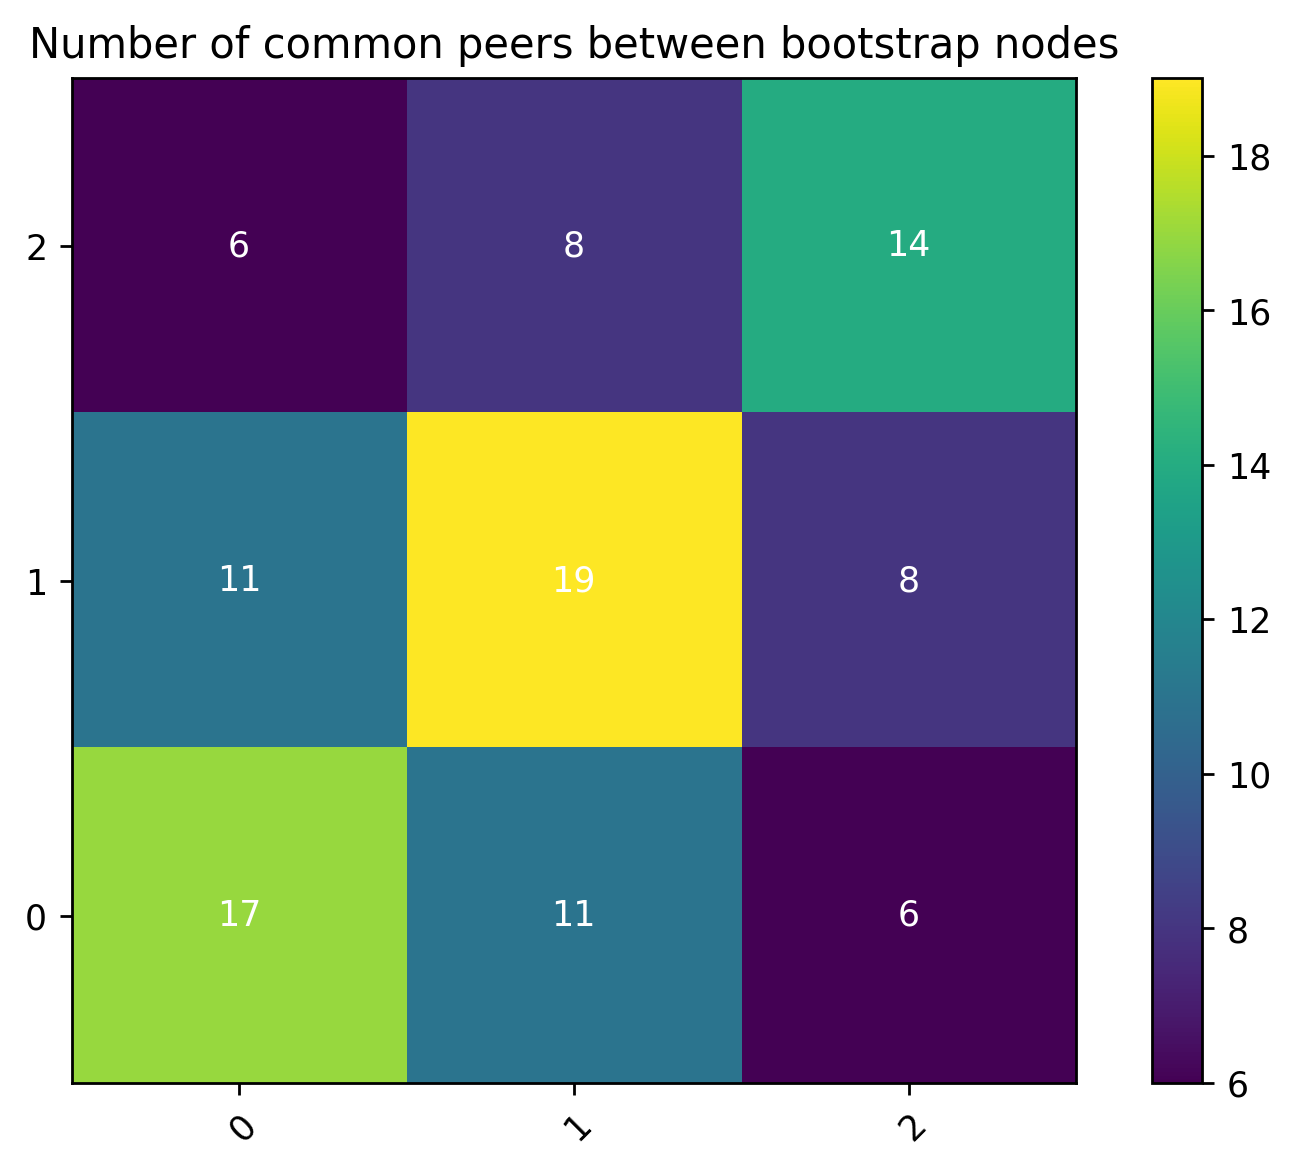
\includegraphics[width=\linewidth]{images/5/5-connectivity.png}
  	\caption{Simulation connectivity}
  	\label{fig:sim-one-duplicates}
   \end{minipage}\hfill
   \begin{minipage}{0.49\textwidth}
     \centering
     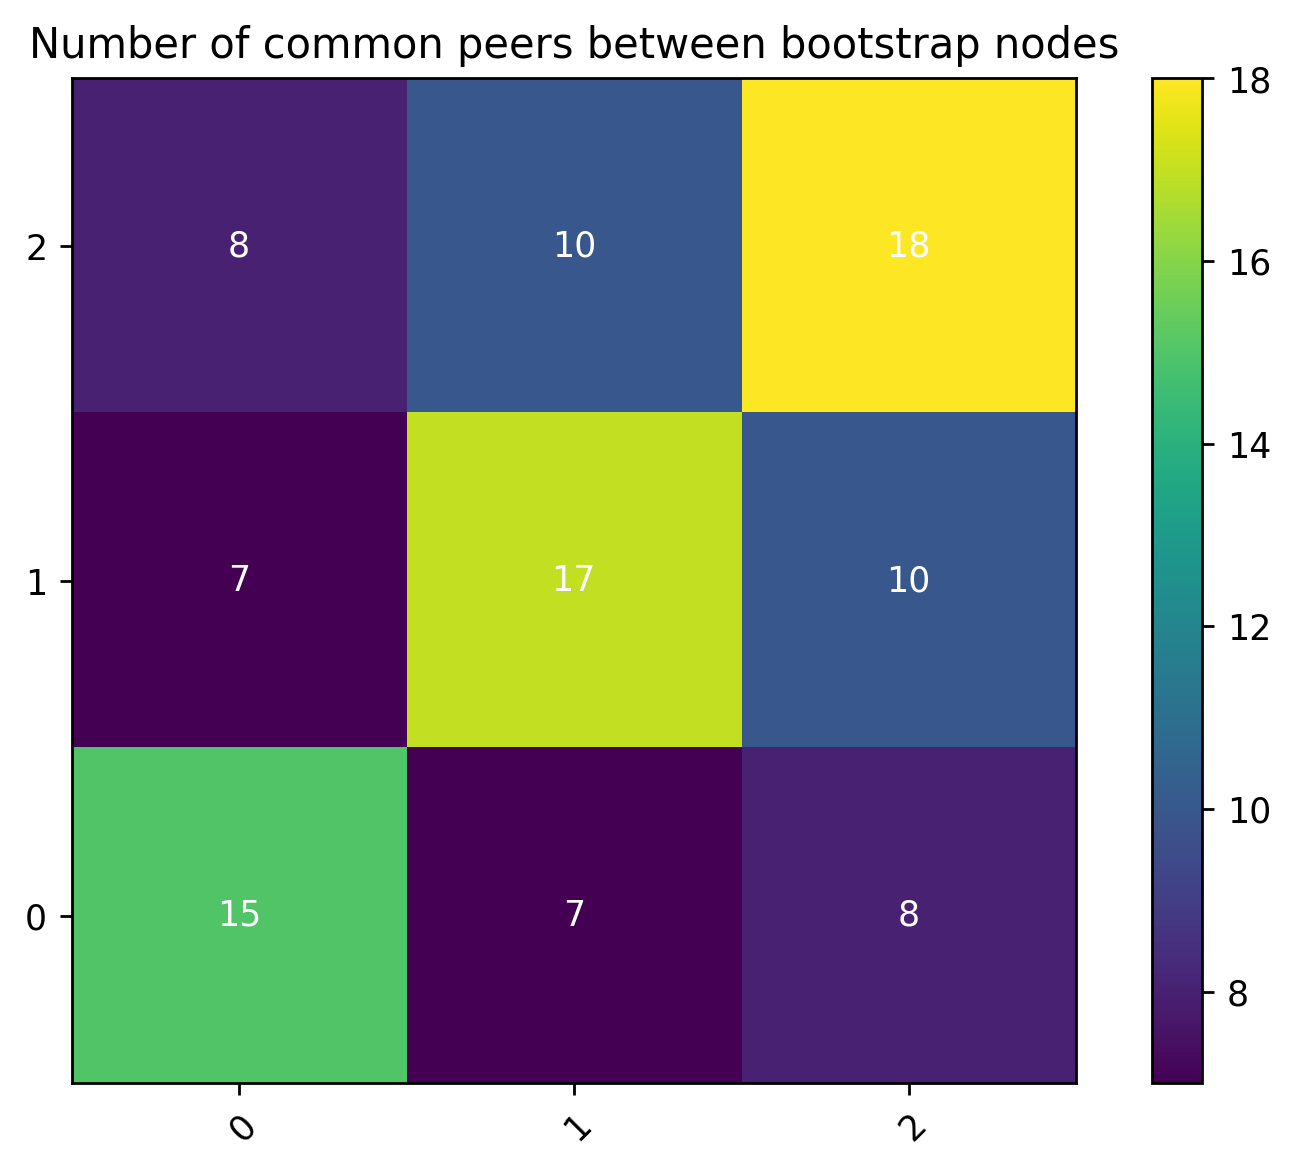
\includegraphics[width=\linewidth]{images/6/6-connectivity.png}
       \caption{Prototype connectivitys}
 		\label{fig:sim-two-duplicates}
   \end{minipage}
\end{figure}

\begin{figure}[H]
   \begin{minipage}{0.49\textwidth}
     \centering
     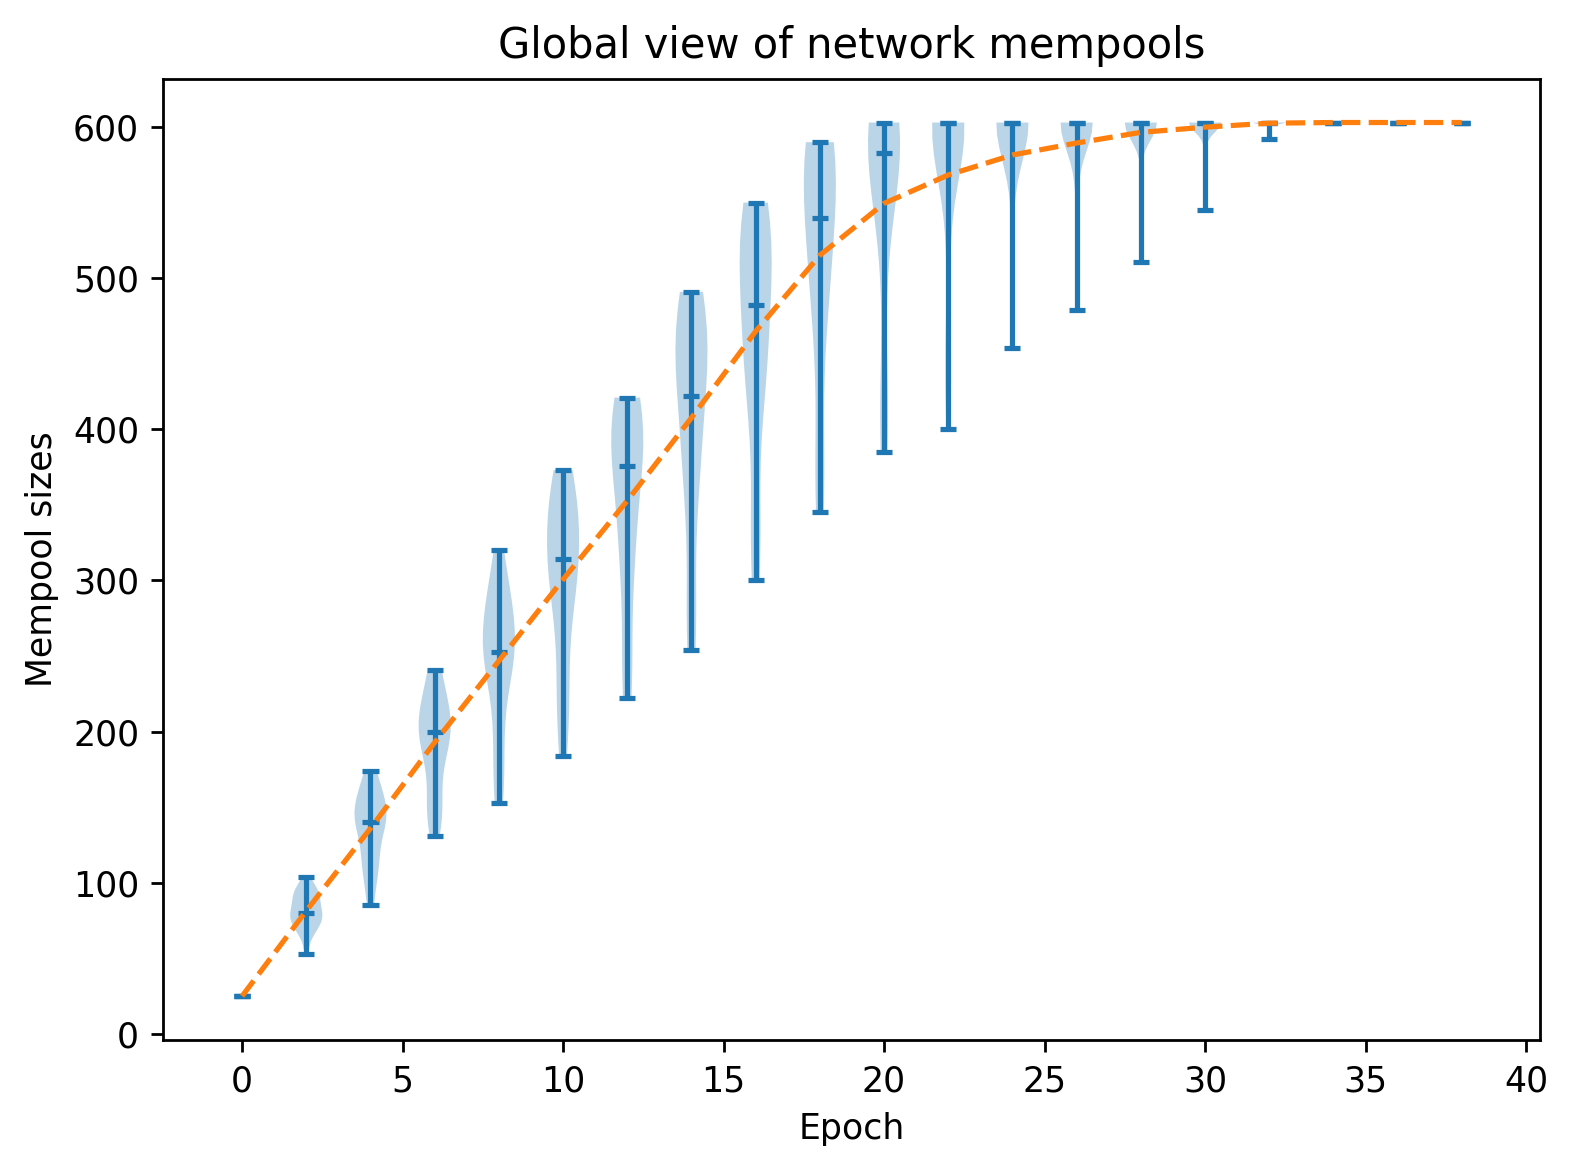
\includegraphics[width=\linewidth]{images/5/5-conv.png}
  	\caption{Simulation convergence rate}
  	\label{fig:sim-one-duplicates}
   \end{minipage}\hfill
   \begin{minipage}{0.49\textwidth}
     \centering
     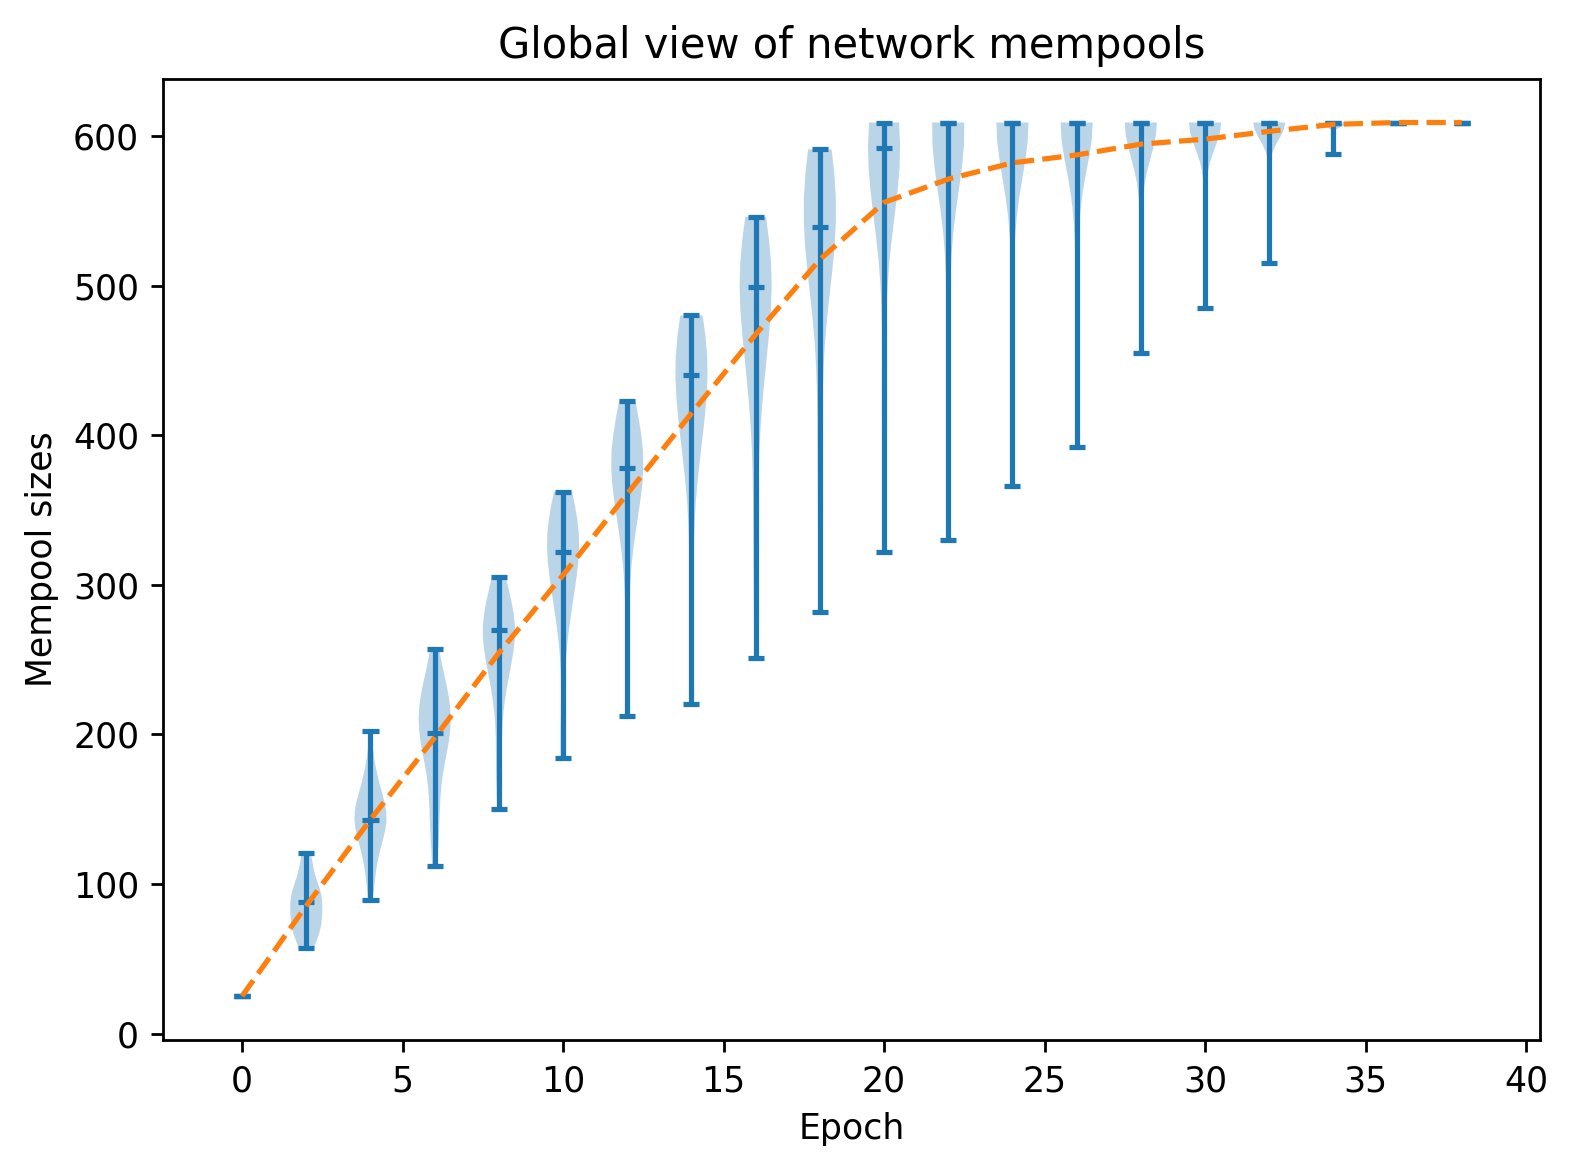
\includegraphics[width=\linewidth]{images/6/6-conv.png}
       \caption{Prototype convergence rate}
 		\label{fig:sim-two-duplicates}
   \end{minipage}
\end{figure}

\begin{figure}[H]
   \begin{minipage}{0.49\textwidth}
     \centering
     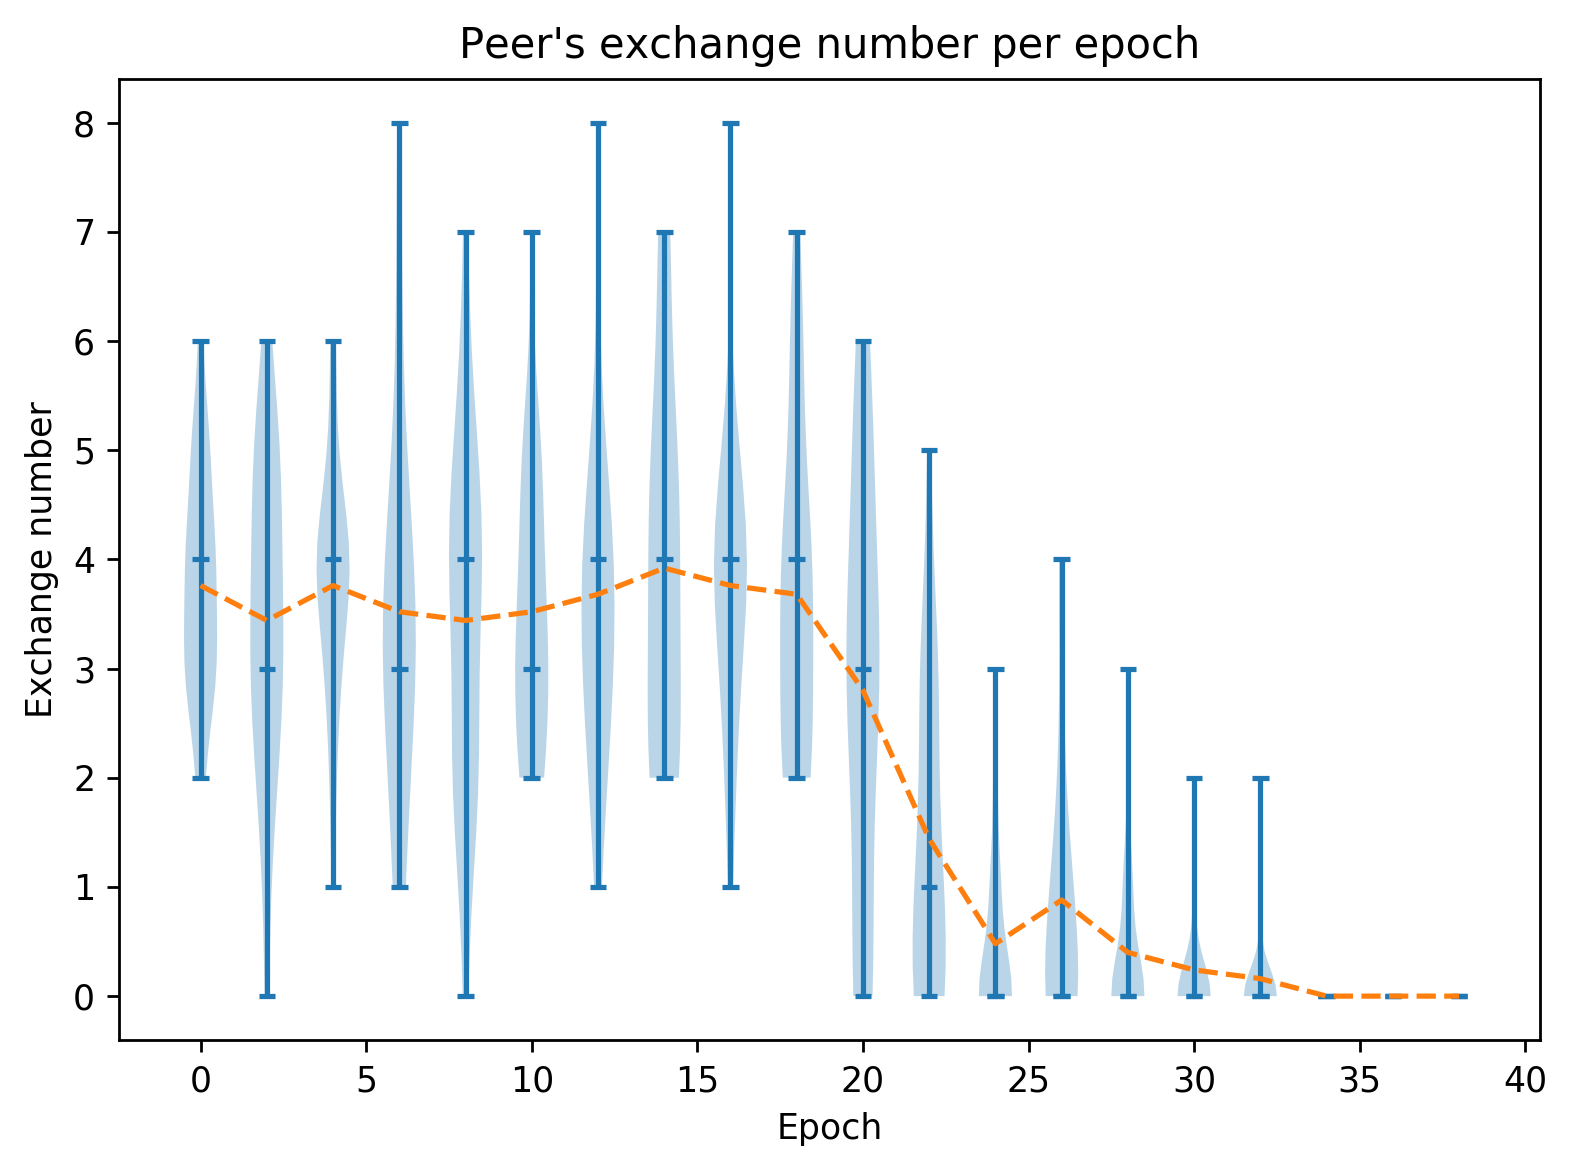
\includegraphics[width=\linewidth]{images/5/5-exchanges.png}
  	\caption{SimulationPrototype exchange per epochs}
  	\label{fig:sim-one-duplicates}
   \end{minipage}\hfill
   \begin{minipage}{0.49\textwidth}
     \centering
     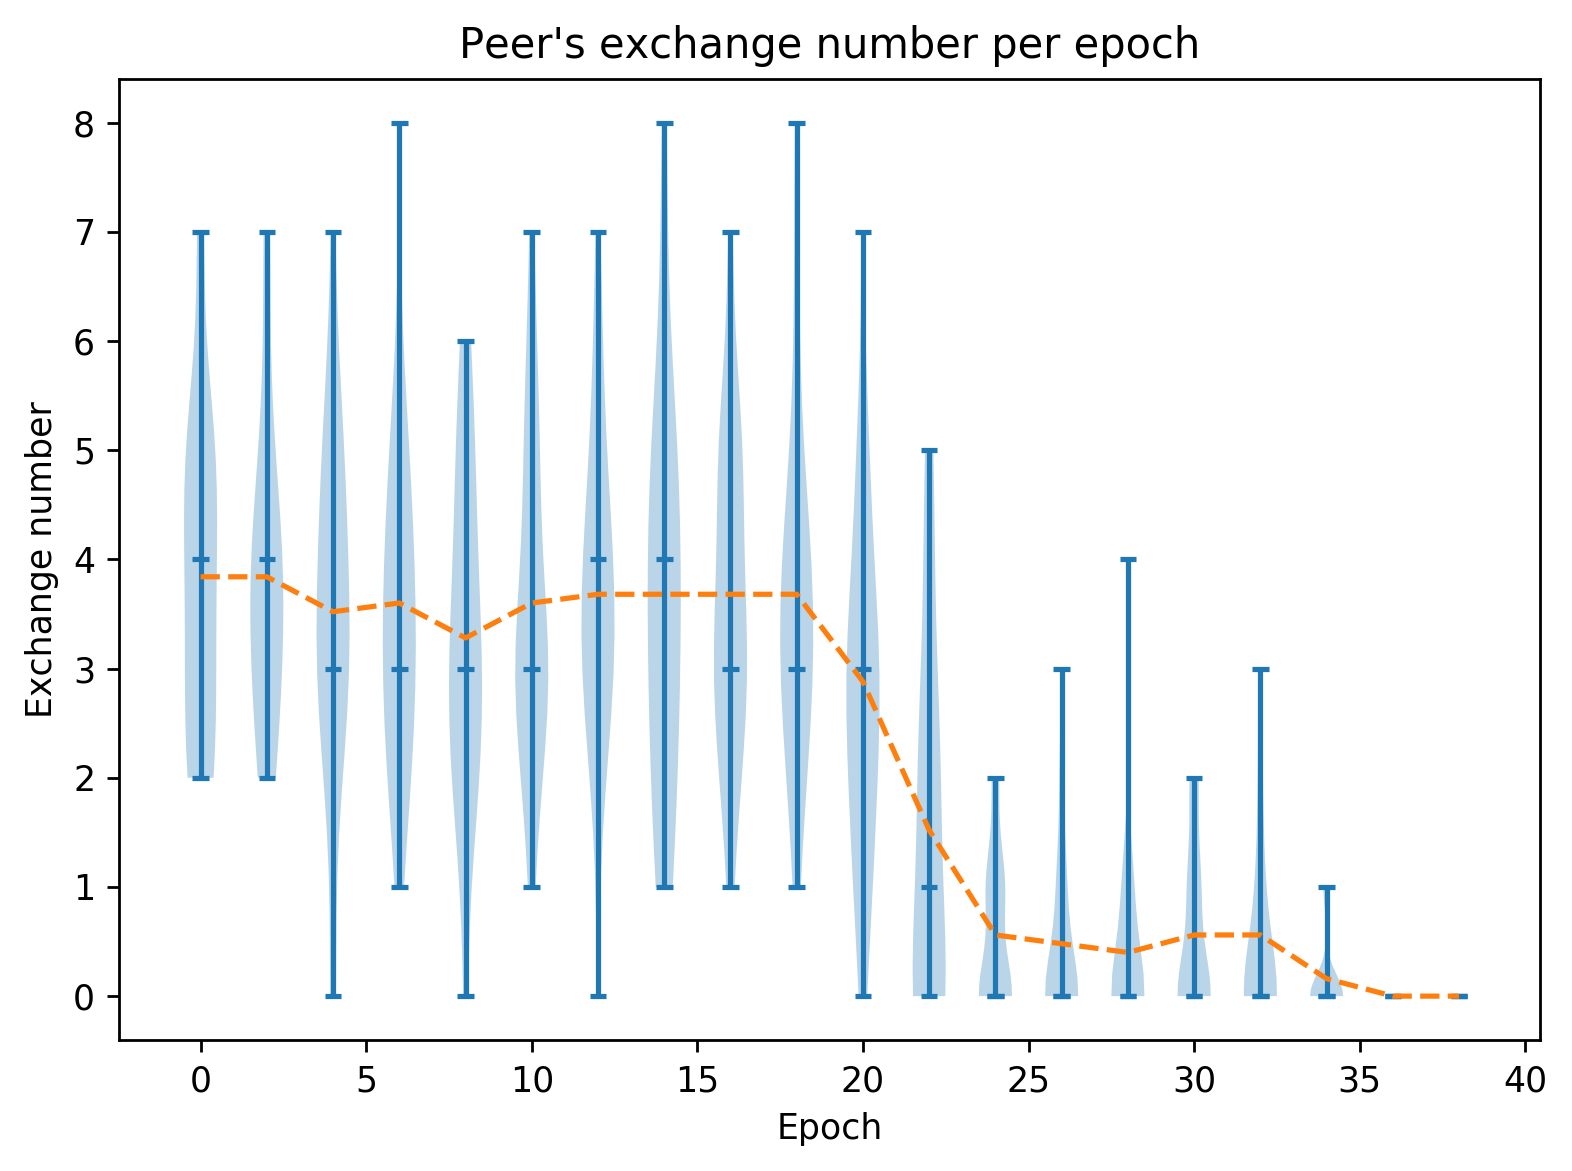
\includegraphics[width=\linewidth]{images/6/6-exchanges.png}
       \caption{Prototype exchange per epoch}
 		\label{fig:sim-two-duplicates}
   \end{minipage}
\end{figure}

\begin{figure}[H]
   \begin{minipage}{0.49\textwidth}
     \centering
     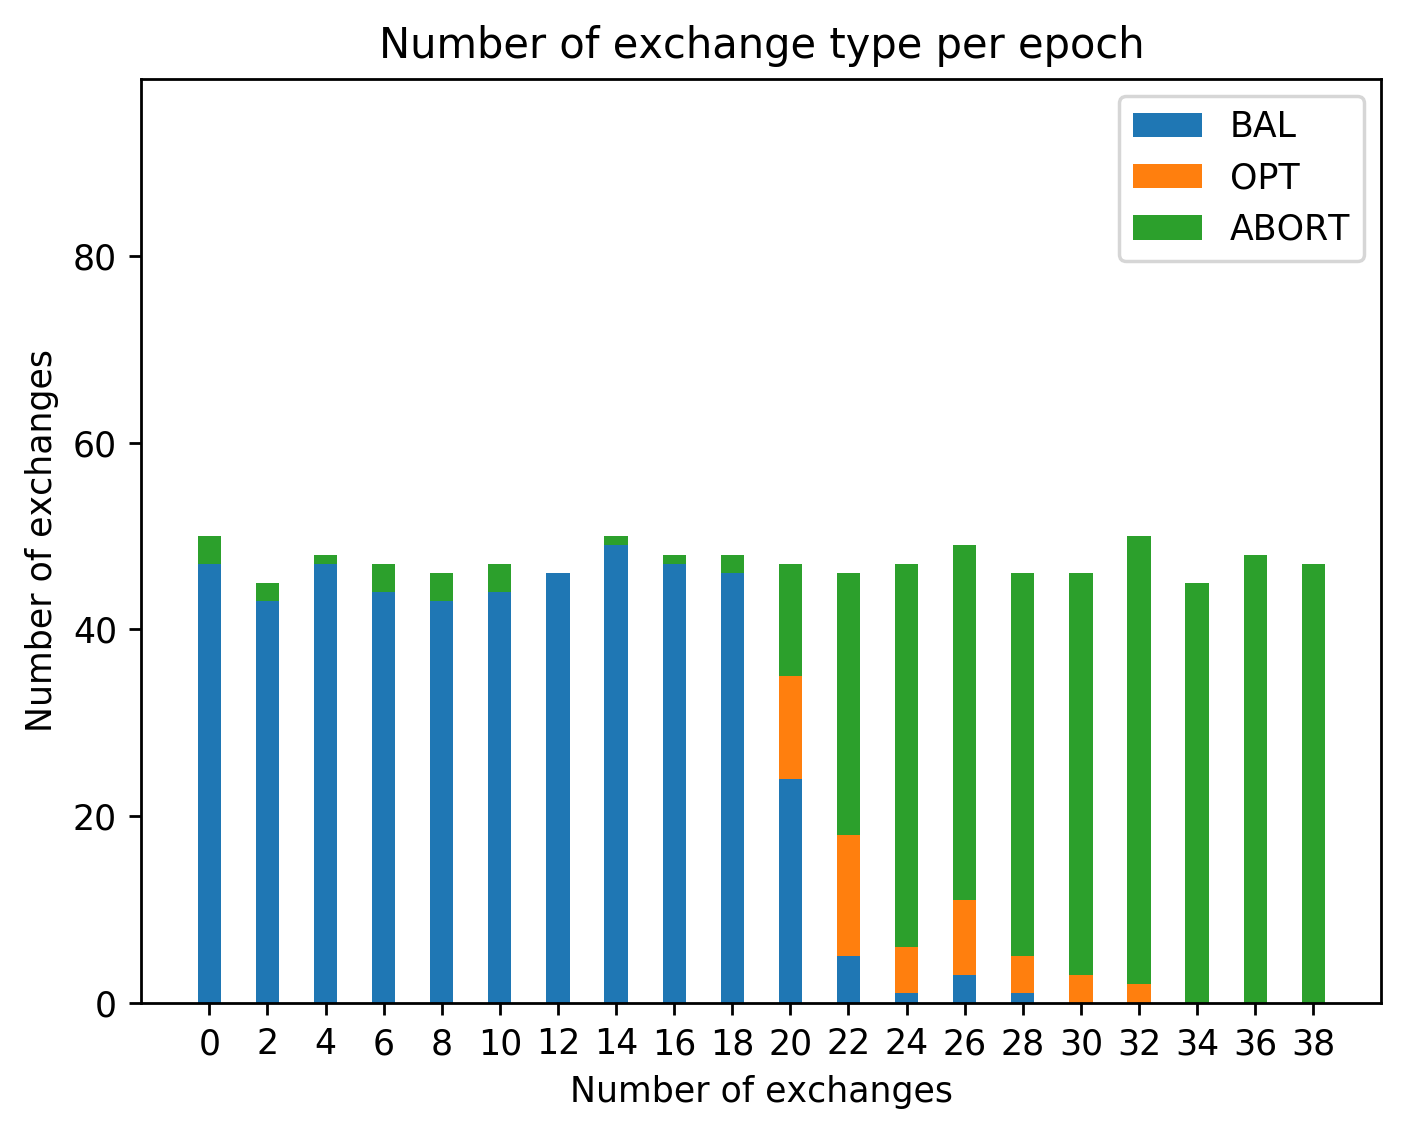
\includegraphics[width=\linewidth]{images/5/5-ex-type.png}
  	\caption{Simulation exchange type per epoch}
  	\label{fig:sim-one-duplicates}
   \end{minipage}\hfill
   \begin{minipage}{0.49\textwidth}
     \centering
     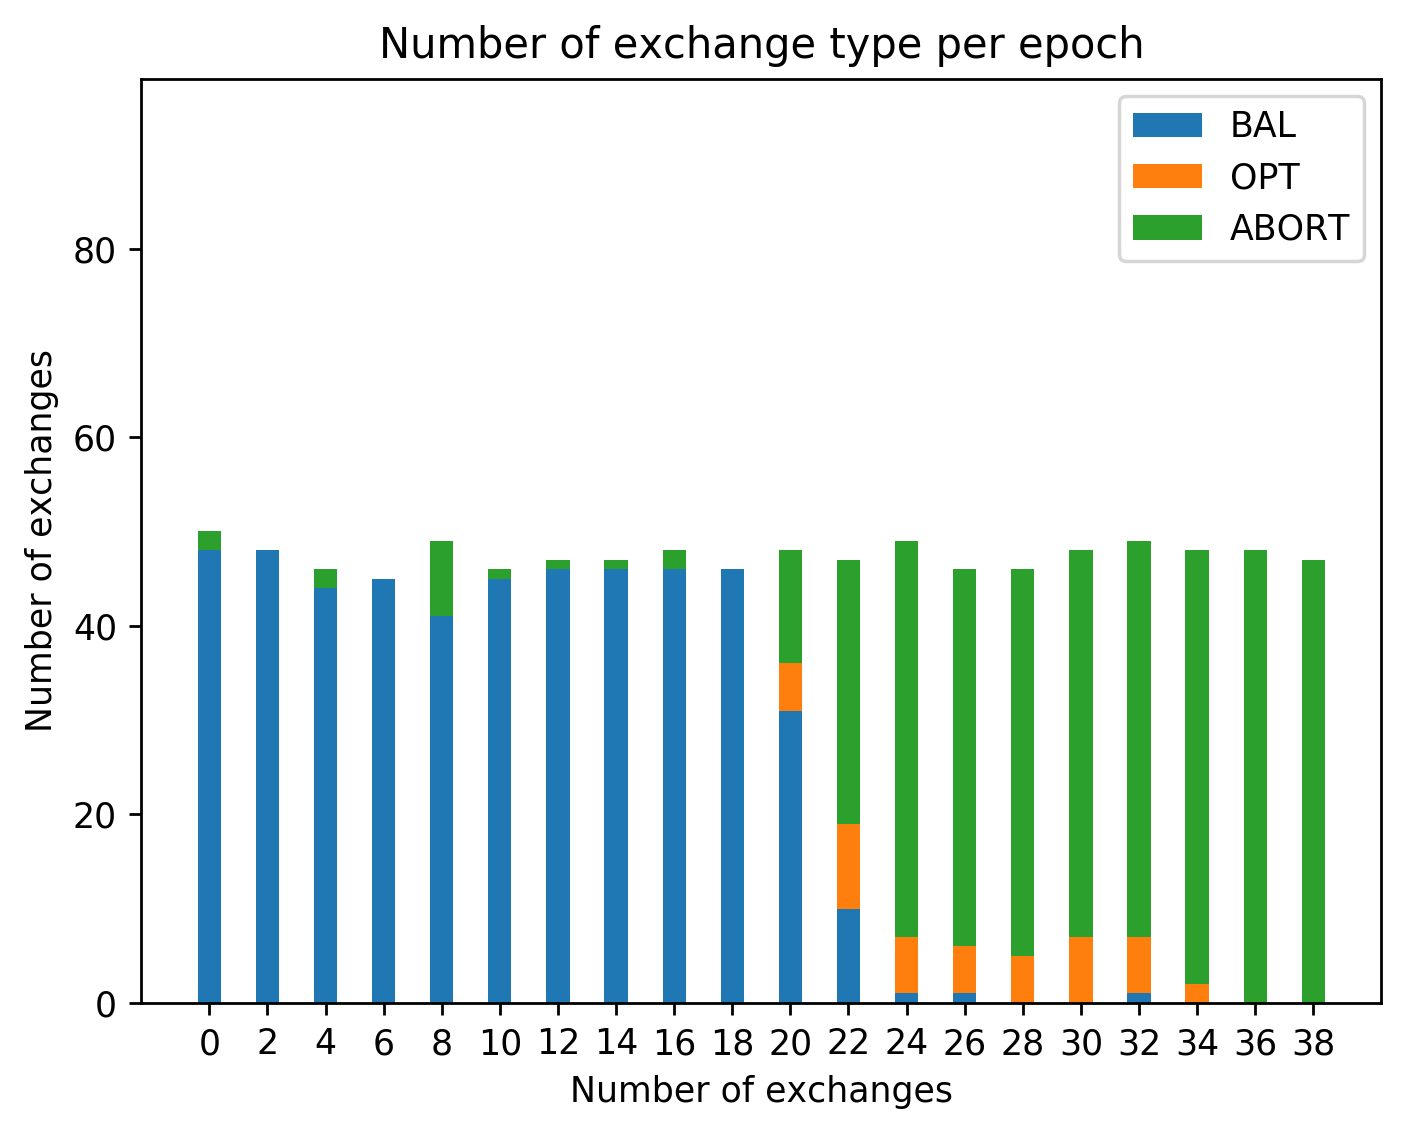
\includegraphics[width=\linewidth]{images/6/6-ex-type}
       \caption{Prototype exchange type per epoch}
 		\label{fig:sim-two-duplicates}
   \end{minipage}
\end{figure}

Most of the metrics in the figures above, show very similar data. Our prototype has a little slower convergence rate and exchange per epoch but this is probably due to small known implementation issues. \\
Still, looking at the plots gives us a high confidence that the simulation can faithfully match a real environment.

\chapter{Experiments}
In this chapter we are going to test the protocol under different assumptions. The parameters taken into account are the following:

\begin{table}[H]
\centering
\resizebox{\textwidth}{!}{%
\begin{tabular}{|l|l|l|}
\hline
                                 & \textbf{Value} & \textbf{Description}                                                  \\ \hline
\textbf{Bootstrap nodes}         & 8              & The number of BNs in the simulation                                   \\ \hline
\textbf{Full nodes}              & 250            & Total number of FN in the simulation. They are ALTRUISTIC by default. \\ \hline
\textbf{Rational nodes}          & Variable       & Percentage of rational nodes                                          \\ \hline
\textbf{Byzantine nodes}         & Variable       & Percentage of byzantine nodes                                         \\ \hline
\textbf{Epochs}                  & 200            & Number of epochs                                                      \\ \hline
\textbf{PoW Difficulty}          & 3              & Difficulty expressed as number of epochs                              \\ \hline
\textbf{Byzantine level}         & 0.4            & Probability for a byzantine node to act byzantine during an exchange  \\ \hline
\textbf{Mempool size}            & 70, 25         & Mean and standard deviation of peer's mempool size                    \\ \hline
\textbf{Number of subscriptions} & Variable       & Number of registration per peer                                       \\ \hline
\textbf{Max BAL exchange}        & 12             & Maximum number of updates per BAL exchange                            \\ \hline
\textbf{Max OPT exchange}        & 20             & Maximum number of updates per OPT exchange                            \\ \hline
\end{tabular}%
}
\caption{Simulation parameters description}
\label{tab:simulation-paramters}
\end{table}

The main goal of these experiments is to see how the protocol behaves under different model such as presence of rational or byzantine or both. We analyze the simulation looking at different factors such as convergence rate, number of duplicate packets, type of exchange, etc. \\
In the end we will also take into consideration some edge cases and see how much the system is resilient against disruption.

\section{Setup}
In the following sections, we will three general simulation in order to see how much the presence of rational and byzantine nodes afflict the system. \\
The parameters of the tree simulation are the following:

\begin{table}[H]
\centering
\resizebox{\textwidth}{!}{%
\begin{tabular}{|l|l|l|l|}
\hline
                                 & \textbf{Simulation One} & \textbf{Simulation two} & \textbf{Simulation 3} \\ \hline
\textbf{Rational nodes}          & 0                       & 100                     & 100                   \\ \hline
\textbf{Byzantine nodes}         & 0                       & 0                       & 50                    \\ \hline
\textbf{Number of subscriptions} & 2                       & 2                       & 2                     \\ \hline
\end{tabular}%
}
\caption{Simulation parameters}
\label{tab:simulation-parameters-two}
\end{table}

Moreover, important factors in the simulation are the connectivity between bootstrap nodes and the number and distribution of node by their nature.

\begin{figure}[!htb]
   \begin{minipage}{0.48\textwidth}
     \centering
     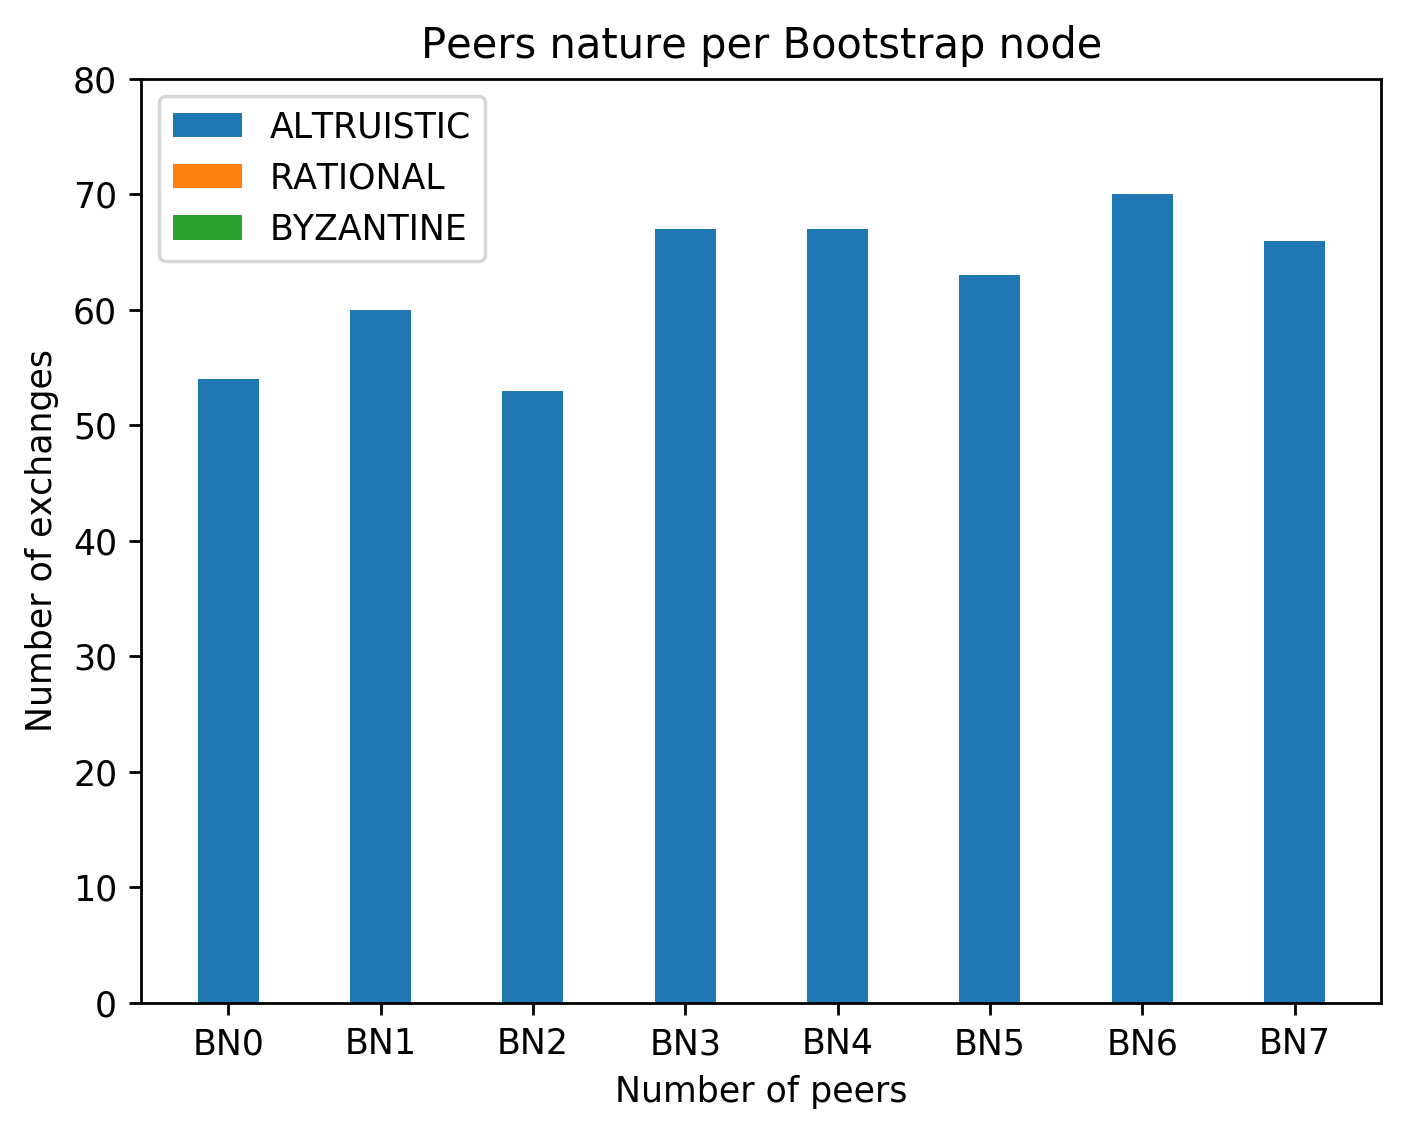
\includegraphics[width=\linewidth]{images/1/1-peer-nature-per-bn.png}
     \caption{First simulation peer distribution and nature}
     \label{fig:sim-one-init-distribution}
   \end{minipage}\hfill
   \begin{minipage}{0.48\textwidth}
     \centering
     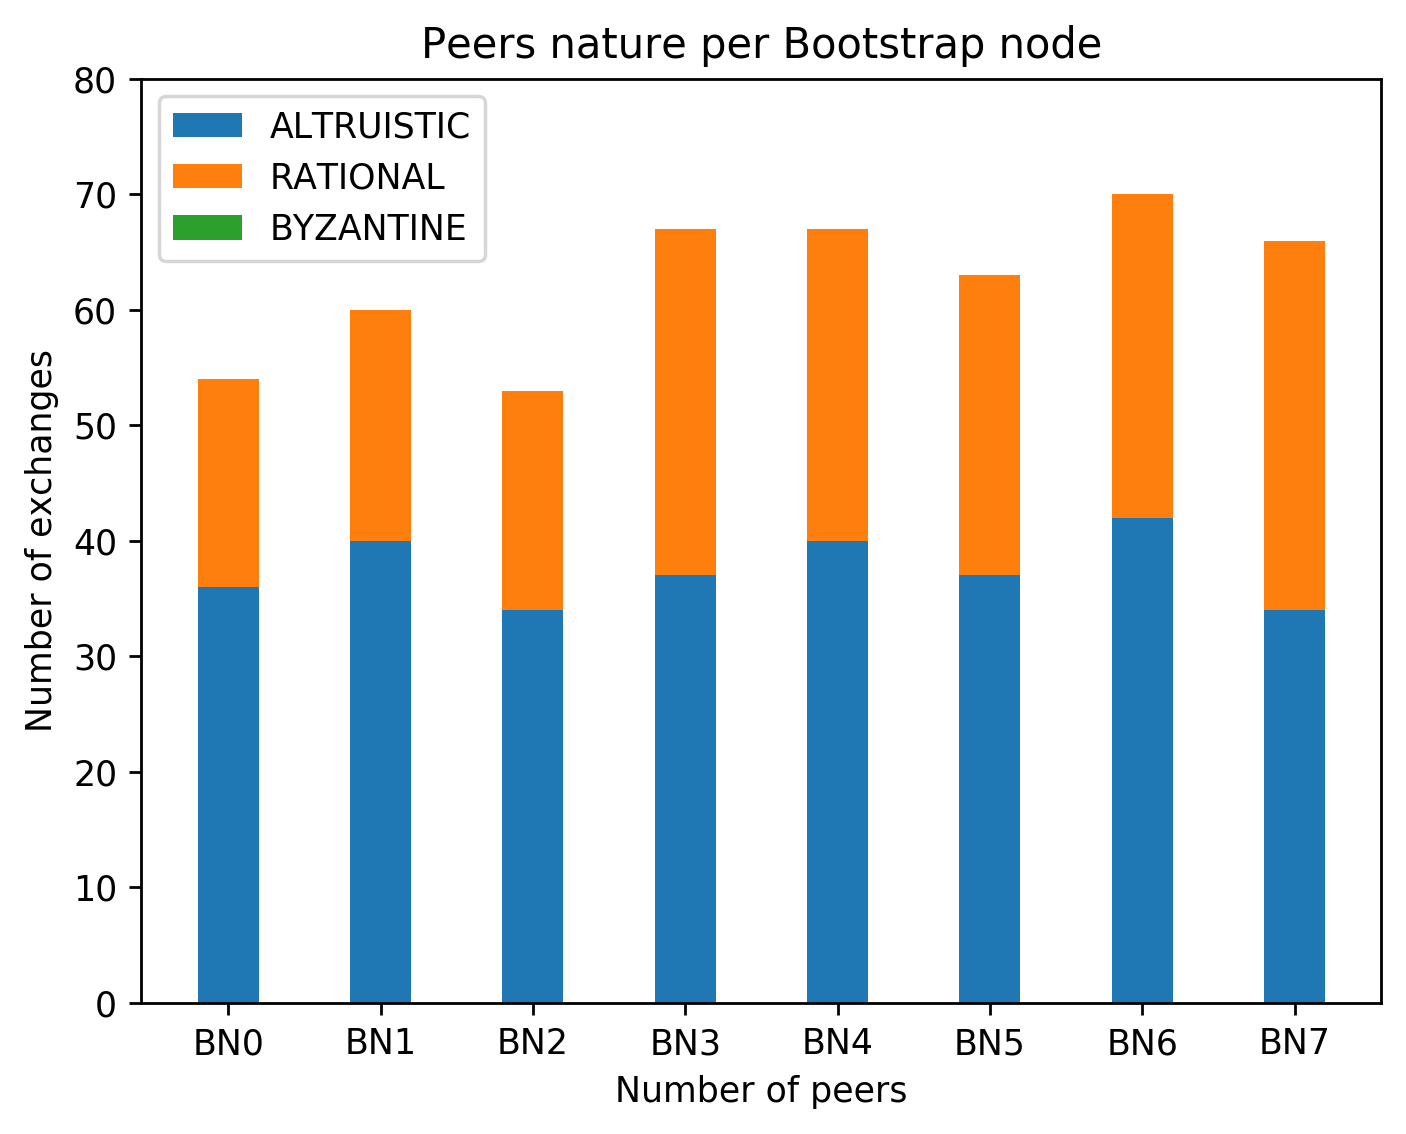
\includegraphics[width=\linewidth]{images/2/two-peer-nature-per-bn.png}
     \caption{Second simulation peer distribution and nature}
     \label{fig:sim-two-init-distribution}
   \end{minipage}
\end{figure}

\begin{figure}[H]
  \centering
  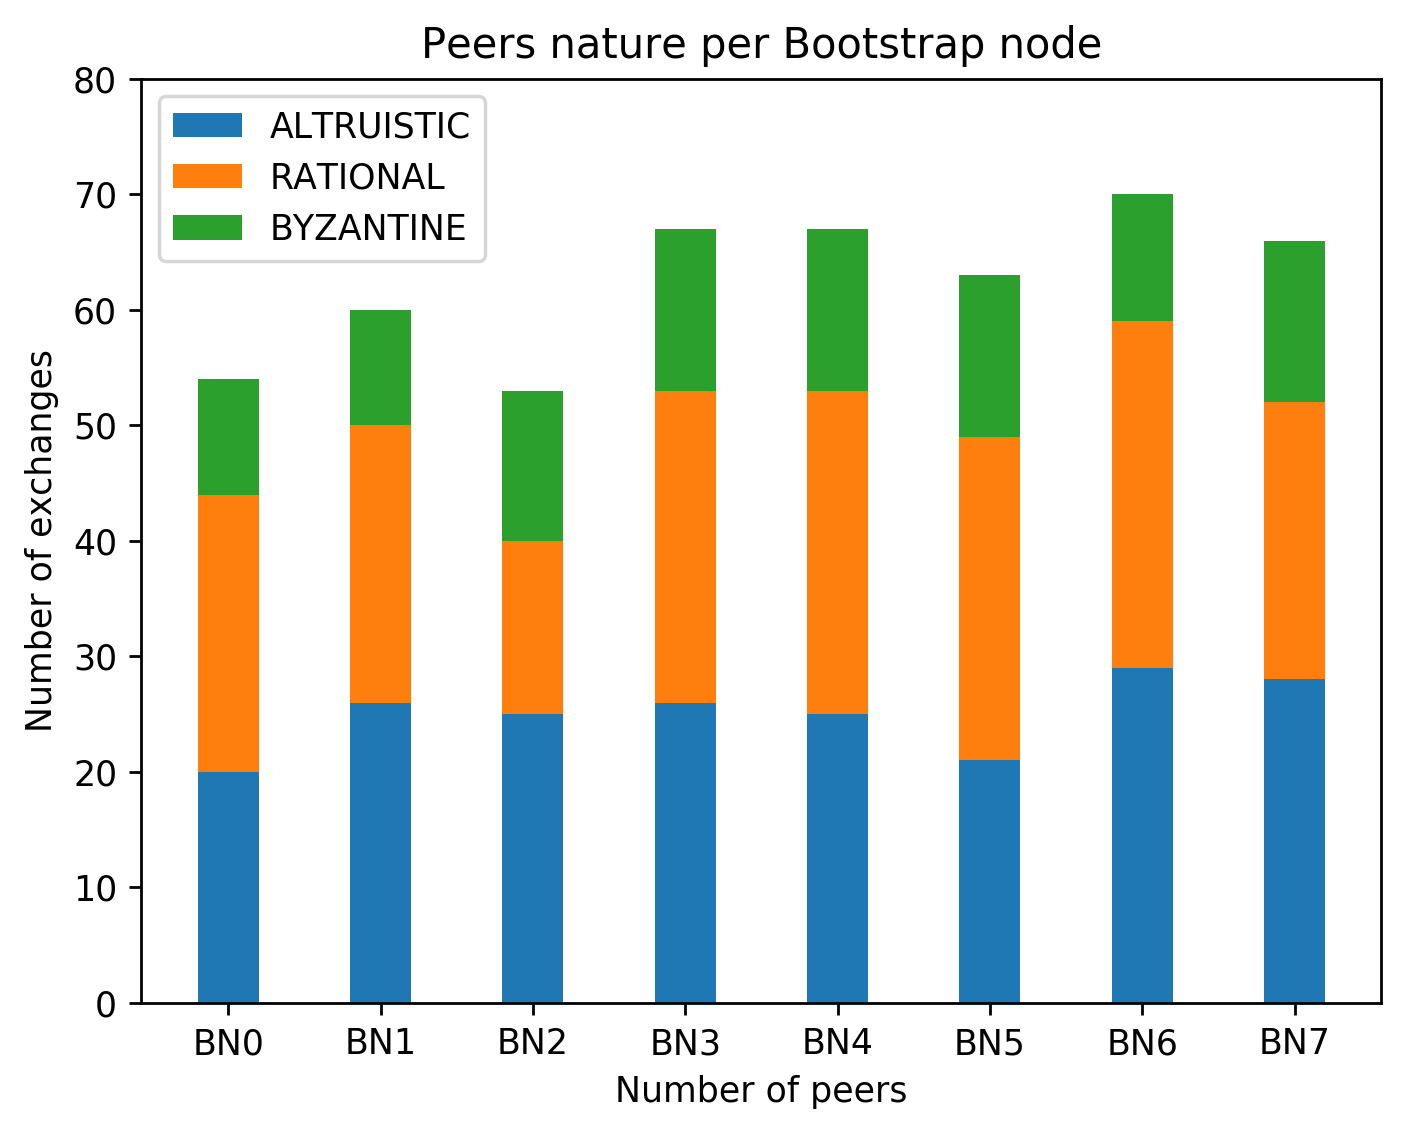
\includegraphics[width=7cm]{images/3/3-peer-nature-per-bn.png}
  \caption{Third simulation peer distribution and nature}
  \label{fig:sim-three-init-distribution}
\end{figure}

As we can see from figure \ref{fig:sim-one-init-distribution}, \ref{fig:sim-two-init-distribution} and \ref{fig:sim-three-init-distribution}, each bootstrap node has more or less the same number of peer and, in the second and first simulation also the distribution of rational and byzantine actors is even. \\

\begin{figure}[H]
  \centering
  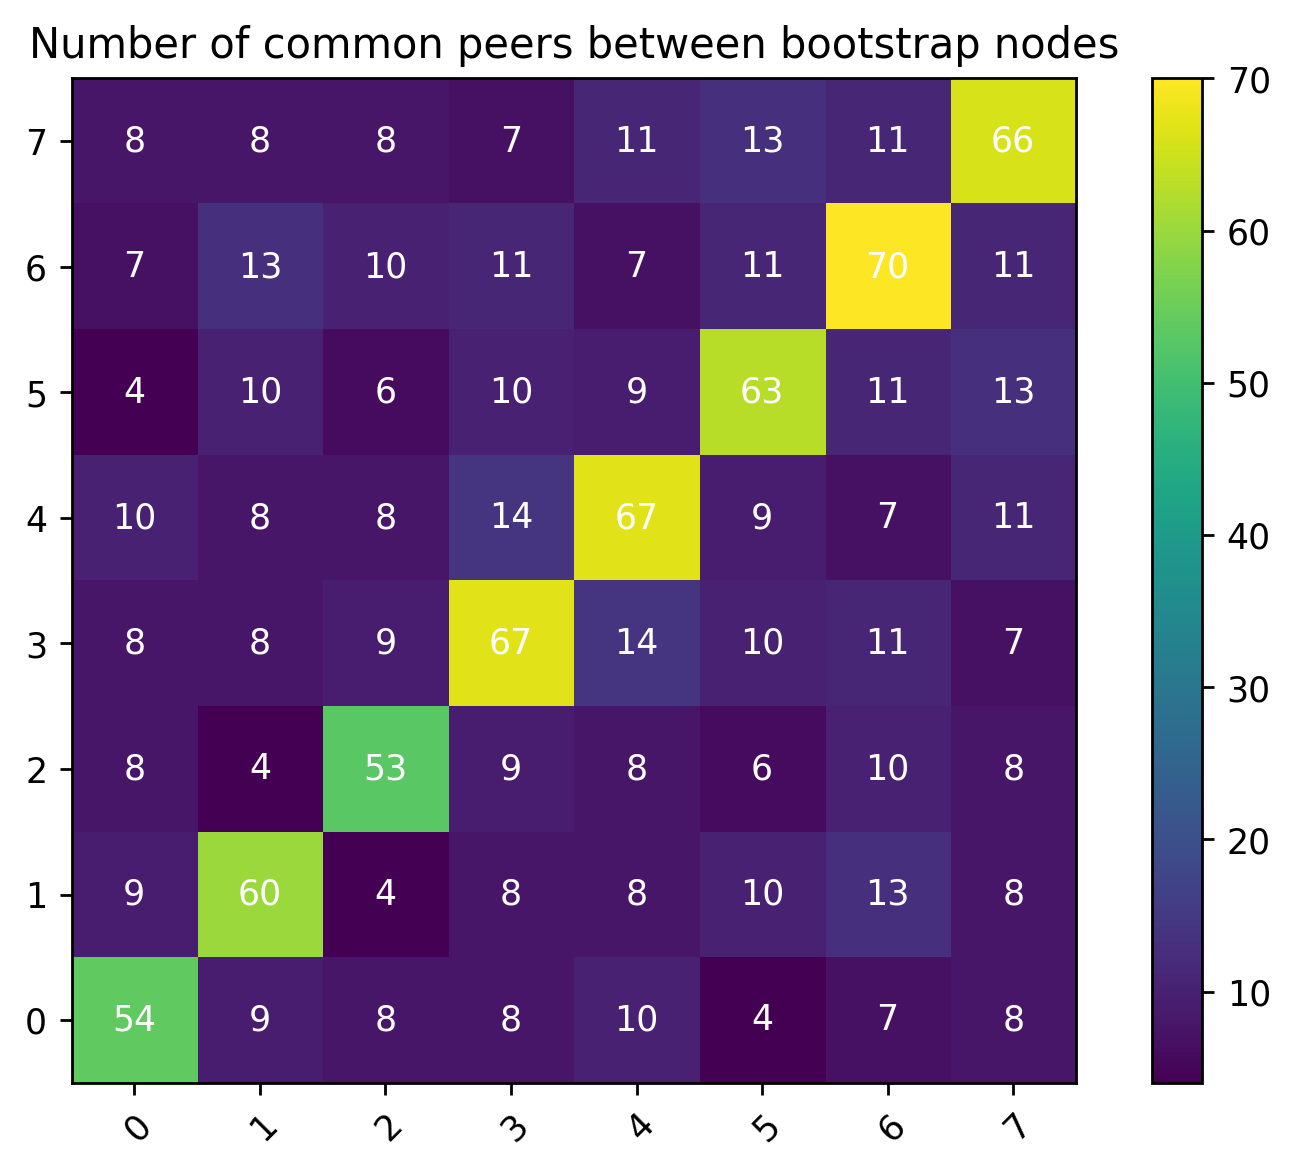
\includegraphics[width=10cm]{images/1/1-connectivity-heatmap.png}
  \caption{Number of peers in common between bootstrap nodes}
  \label{fig:connectivity-general}
\end{figure}

Moreover, from figure \ref{fig:connectivity-general}, we can also see that each bootstrap node has a connection with all the other bootstrap node meaning that the network is fully connected. This is a needed condition in order for the protocol to work. 

\section{Convergences rate}
The first propriety we want to analyze is the converge rate. 

\begin{figure}[!htb]
   \begin{minipage}{0.49\textwidth}
     \centering
     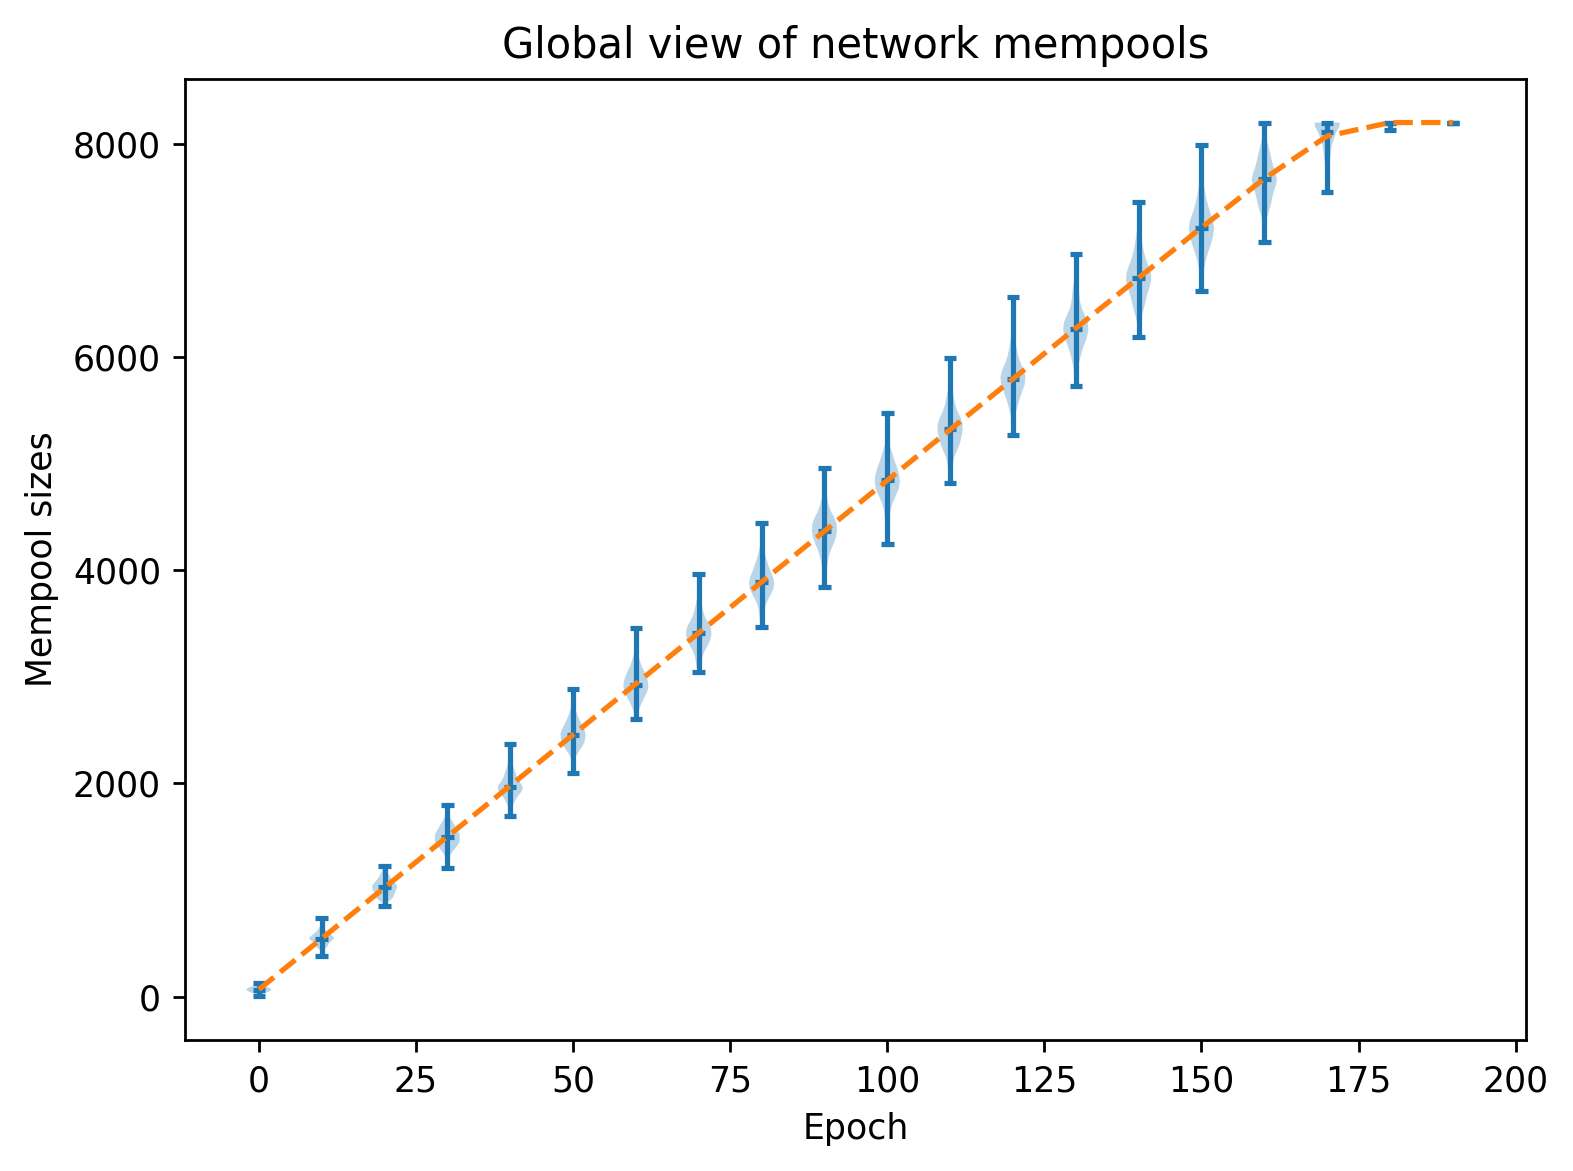
\includegraphics[width=\linewidth]{images/1/1-convergence.png}
  	\caption{1st simulation convergence rate}
  	\label{fig:sim-one-conv}
   \end{minipage}\hfill
   \begin{minipage}{0.49\textwidth}
     \centering
     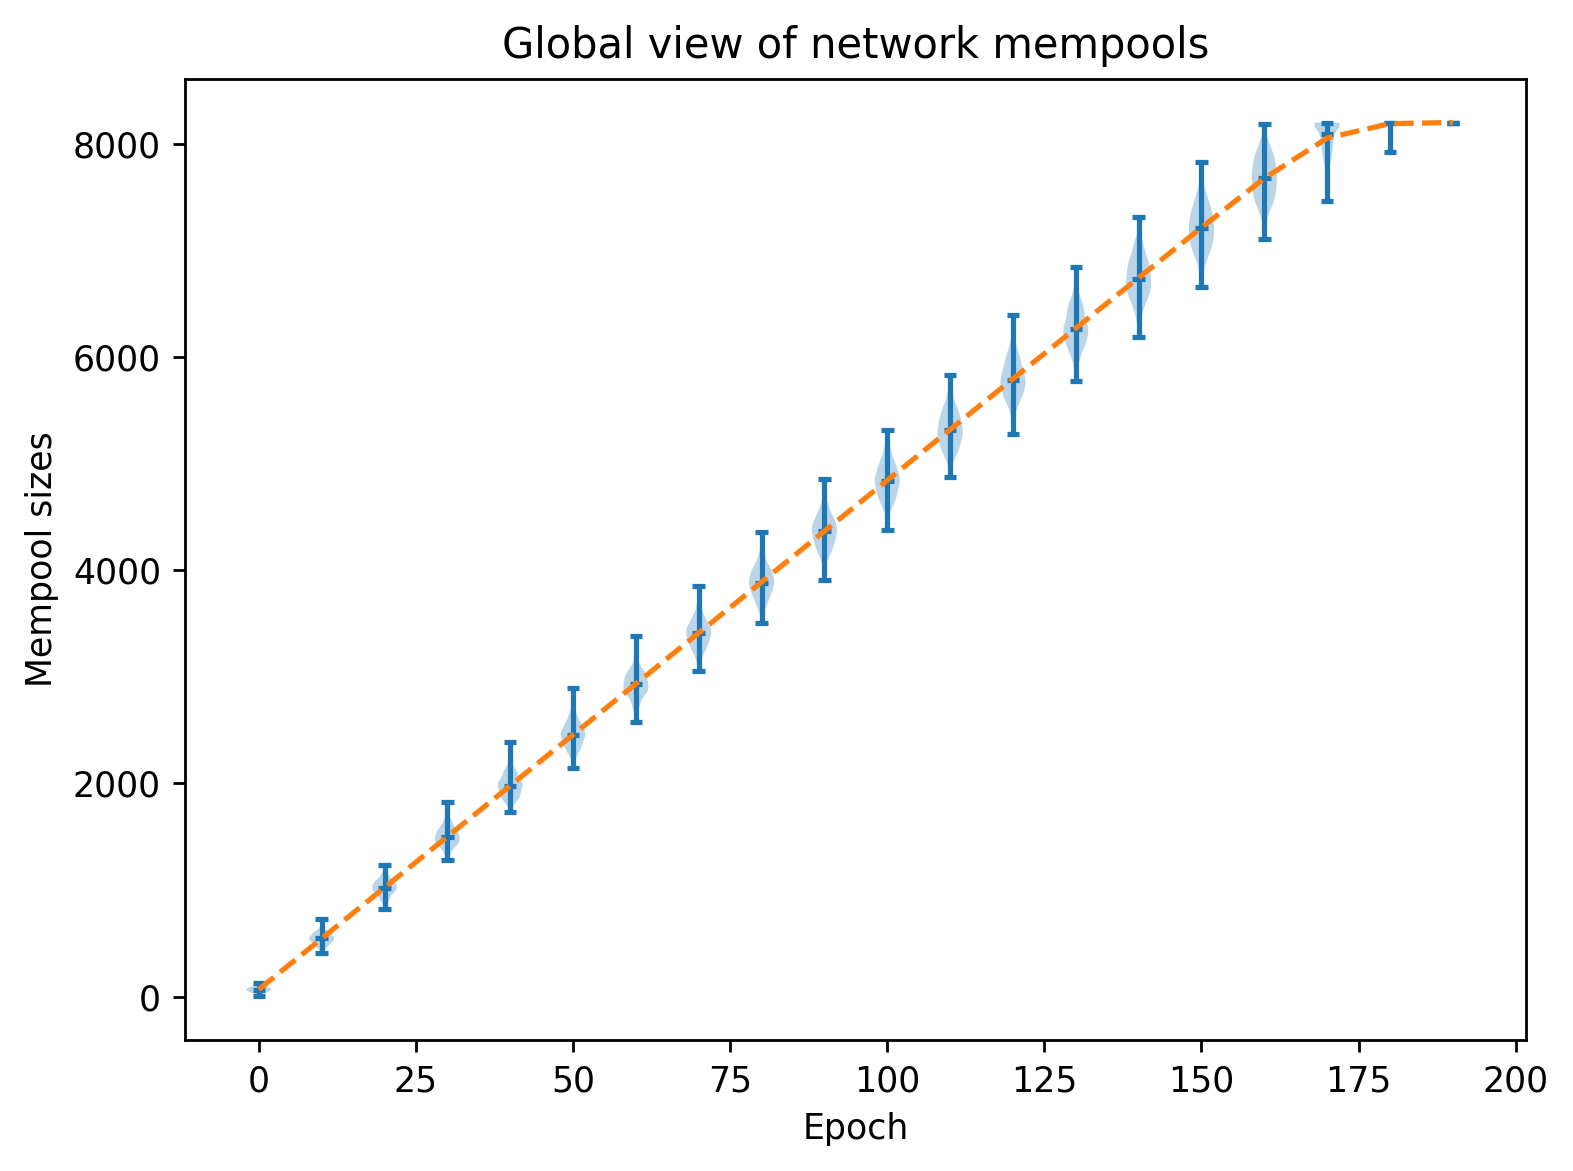
\includegraphics[width=\linewidth]{images/2/two-convergence.png}
       \caption{2nd simulation convergence rate}
 		\label{fig:sim-two-conv}
   \end{minipage}
\end{figure}

\begin{figure}[H]
  \centering
  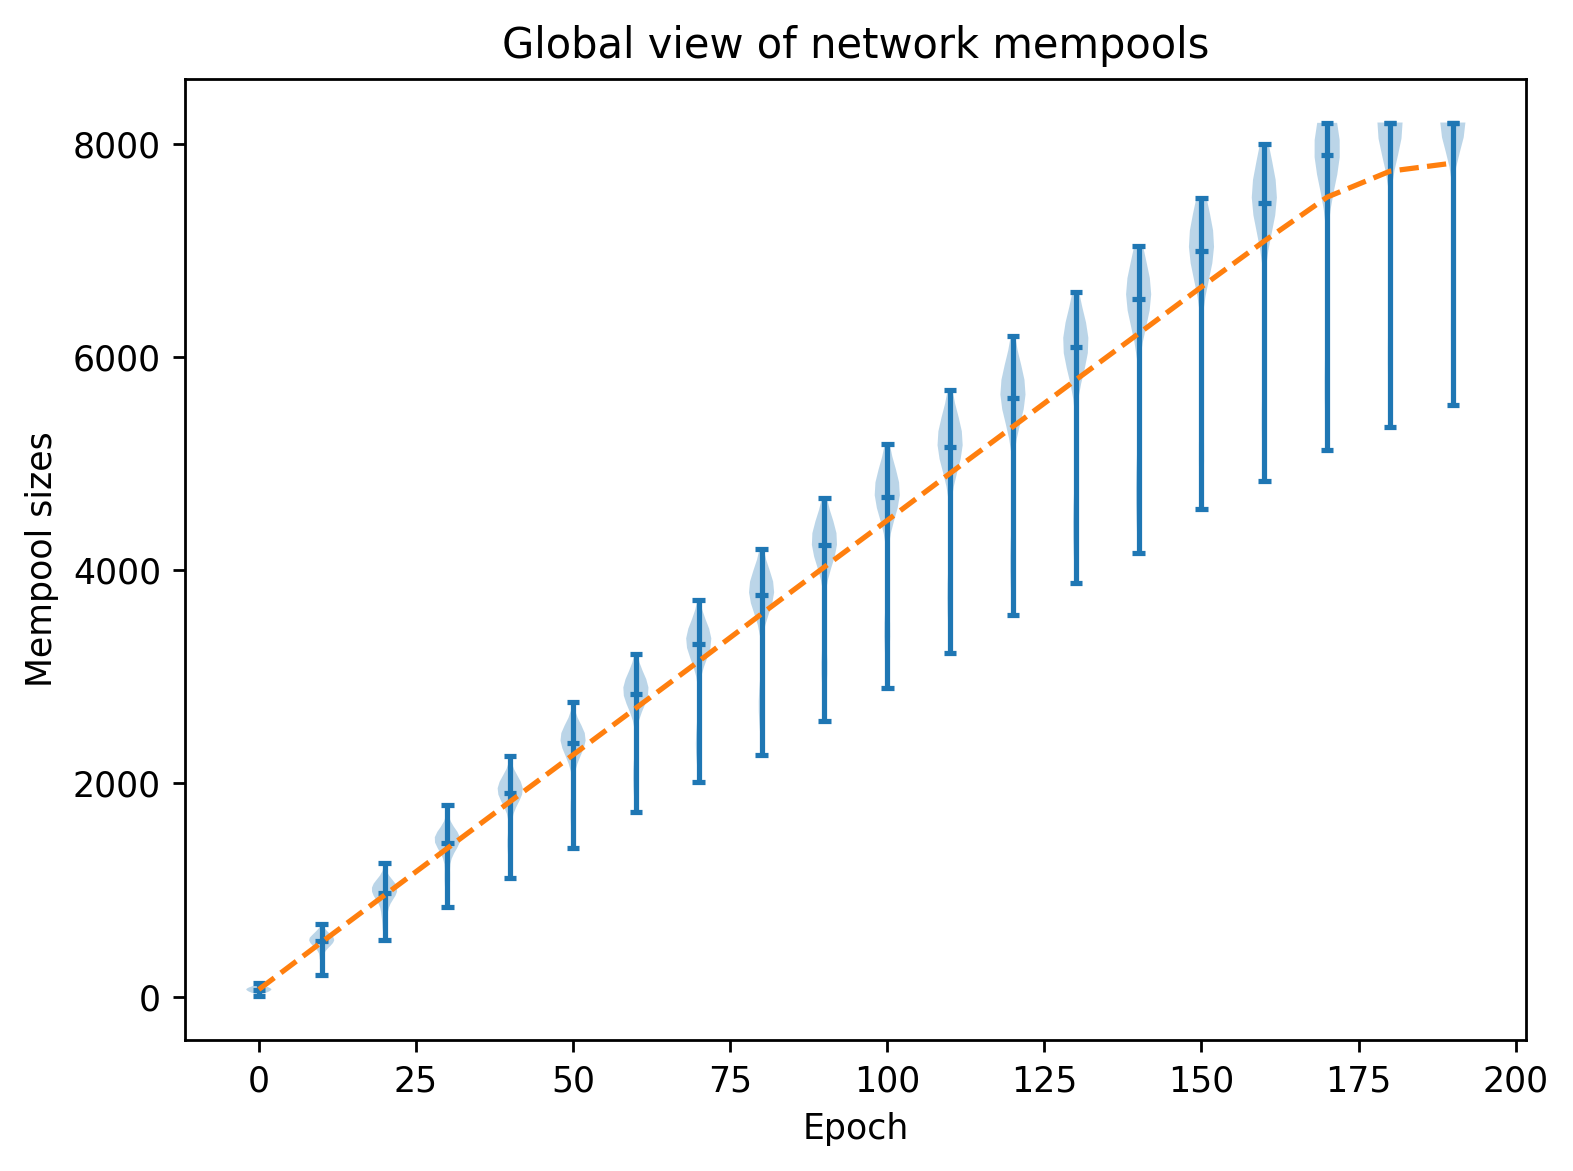
\includegraphics[width=7cm]{images/3/3-convergence.png}
  \caption{3rd simulation converge rate}
  \label{fig:sim-three-conv}
\end{figure}


As we can see from figures \ref{fig:sim-one-conv} and \ref{fig:sim-two-conv}, the presence of rational nodes does not affect the convergence rate at all until the last 20 epochs. This sounds reasonable as peer's mempool are going to be more full and OPT messages help peers get the last missing updates if they don't have anything to share. Since rational nodes don't accept OPT exchanges, full network convergence is more difficult to reach. \\
The situation change n figure \ref{fig:sim-three-conv}, when byzantine actors are introduced. In the last figure we can clearly see that more peers are having a hard time receiving updates and in 200 epochs are not enough to reach the same level of convergence of the previous situations. Still, even if more peers are having troubles, most of them (as shown in the distribution of bars) have a mempool size above the mean. 
\section{Duplicates}
As we want to avoid wasting resources, an important metrics is the number of duplicates updates received.

\begin{figure}[!htb]
   \begin{minipage}{0.49\textwidth}
     \centering
     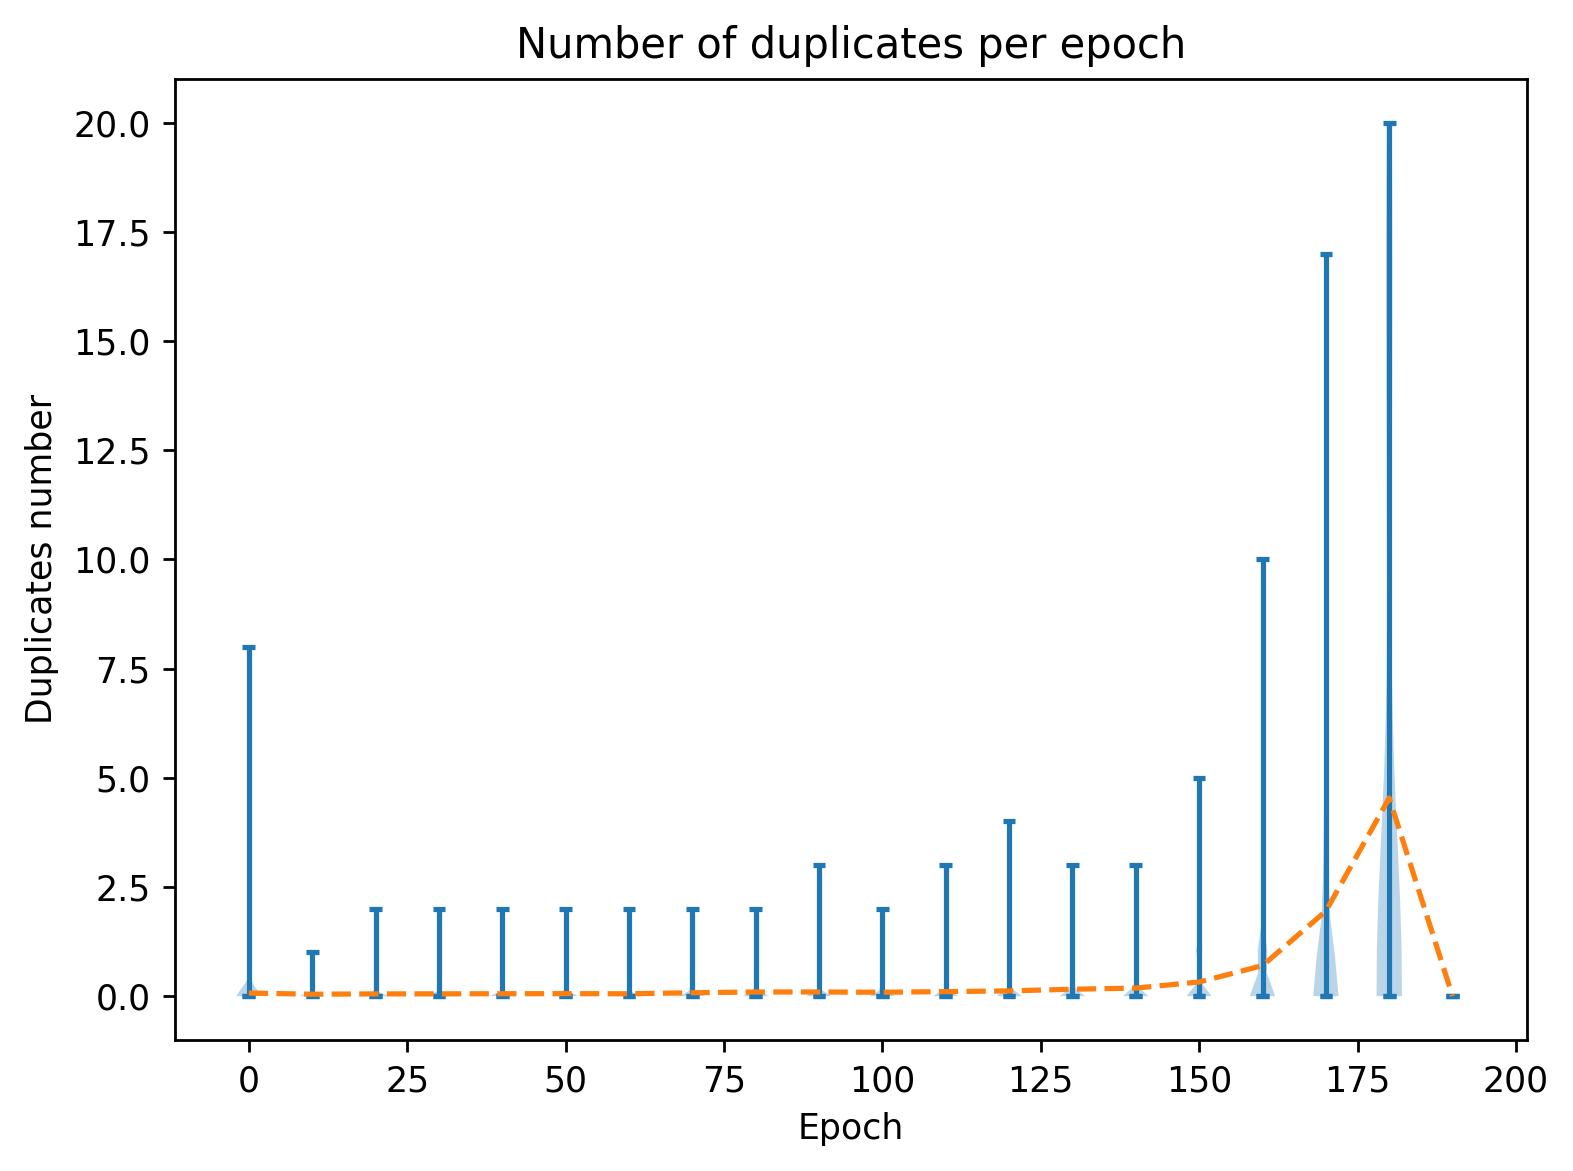
\includegraphics[width=\linewidth]{images/1/1-duplicates.png}
  	\caption{1st simulation duplicates updates}
  	\label{fig:sim-one-duplicates}
   \end{minipage}\hfill
   \begin{minipage}{0.49\textwidth}
     \centering
     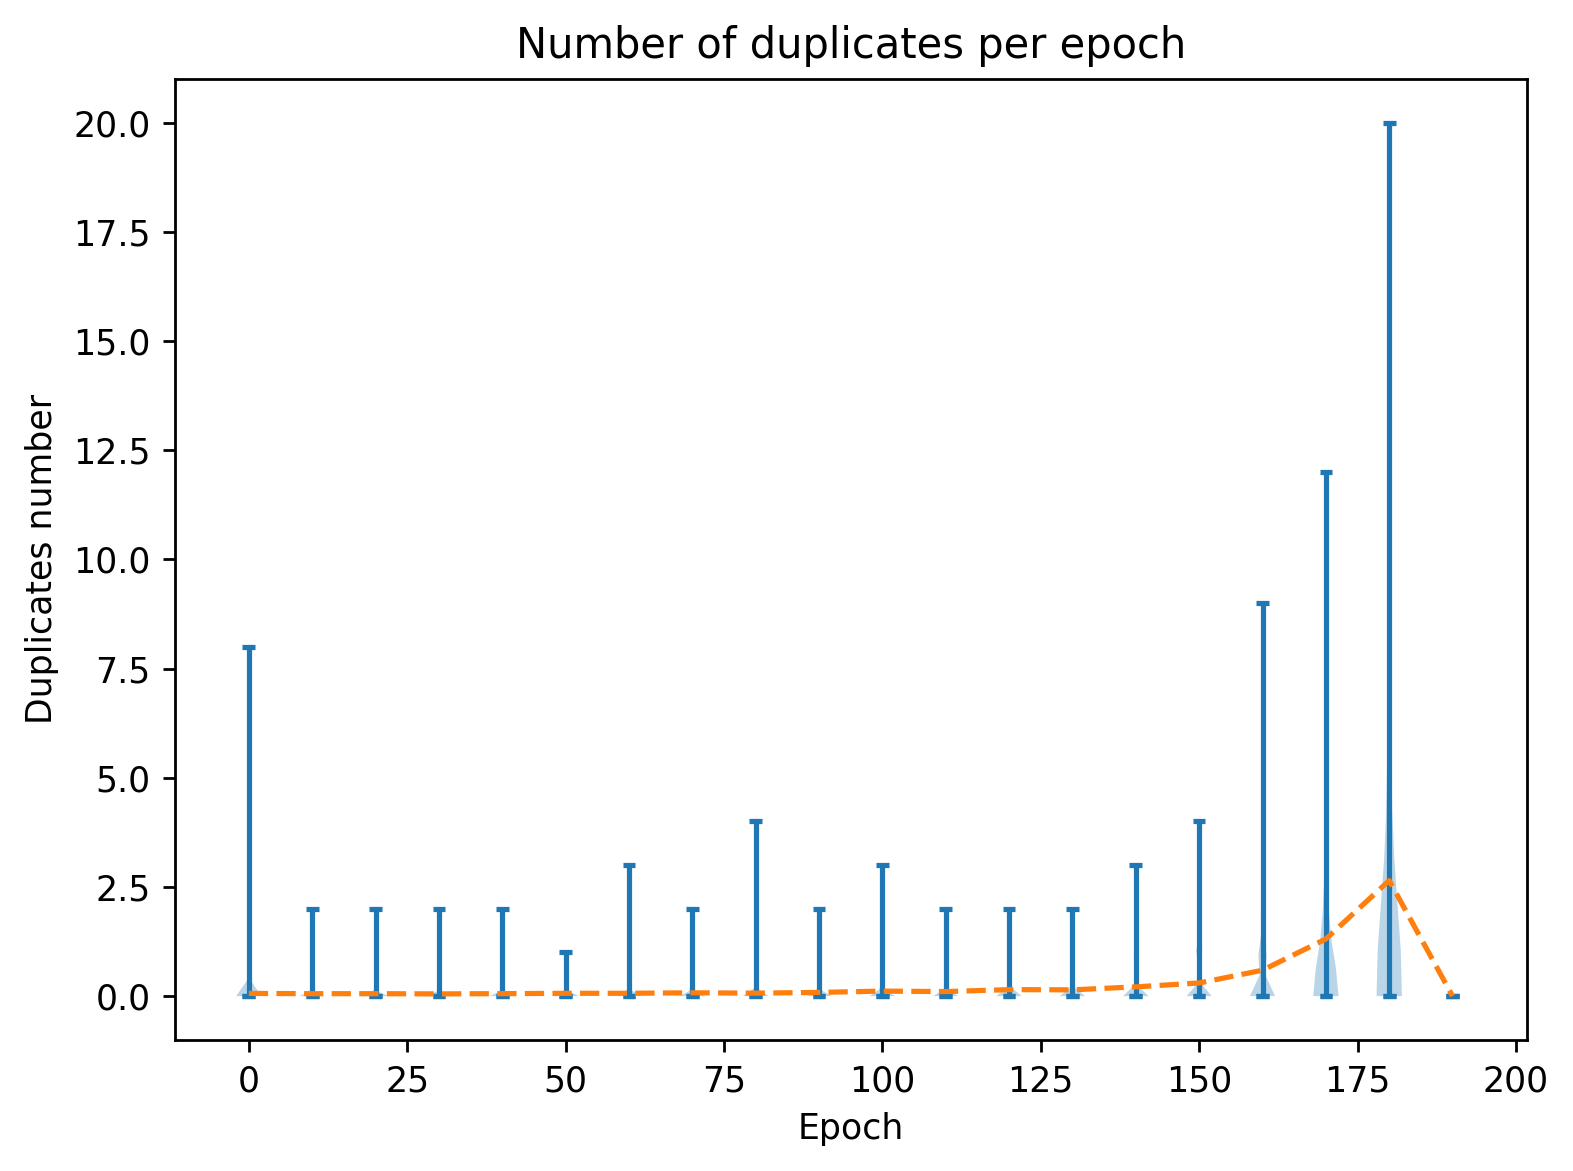
\includegraphics[width=\linewidth]{images/2/two-duplicates.png}
       \caption{2nd simulation duplicates updates}
 		\label{fig:sim-two-duplicates}
   \end{minipage}
\end{figure}

\begin{figure}[H]
  \centering
  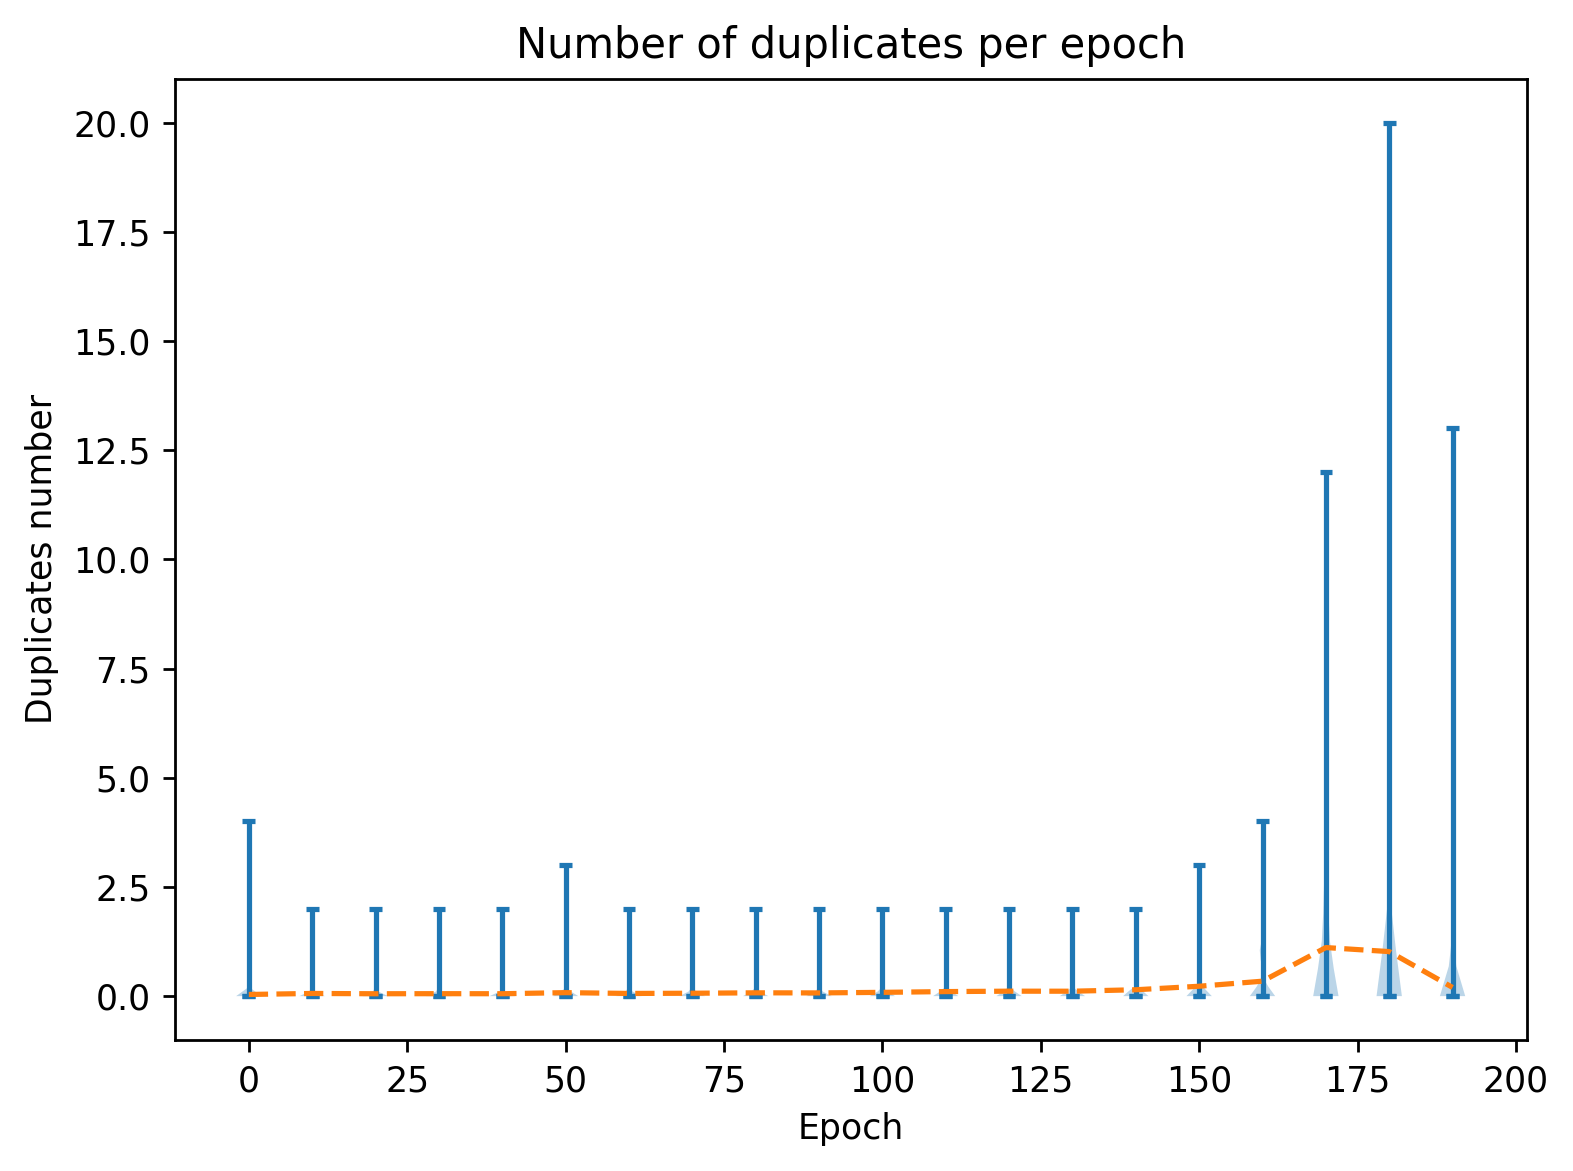
\includegraphics[width=7cm]{images/3/3-duplicates.png}
  \caption{3rd simulation duplicates updates}
  \label{fig:sim-three-duplicates}
\end{figure}

As we can see from figures \ref{fig:sim-one-duplicates}, \ref{fig:sim-two-duplicates}, and \ref{fig:sim-three-duplicates} the number of duplicates updates tends to be higher in the final steps of the simulations. This is because mempools are becoming fuller and so, since peers exchange updates concurrently, there is higher probability to receive a duplicate. \\
Moreover, as more byzantine and rational peer are introduces in the network, number of duplicates mean also decrease. This is because less exchange are made as rational peers don't accept OPT messages and byzantine have a probability of invalidating the exchange. \\
Still, even if the mean in the last figure is lower than in the other two, we have to remember that the third simulation wasn't able to reach full network convergence.

\section{Exchange types}
Another crucial metrics is the percentage of BAL exchange versus OPT and ABORT. Since we want to incentivise peers to execute, as much as possible, the tic-for-tac trade we need to see if our simulations support this requirements.

\begin{figure}[!htb]
   \begin{minipage}{0.49\textwidth}
     \centering
     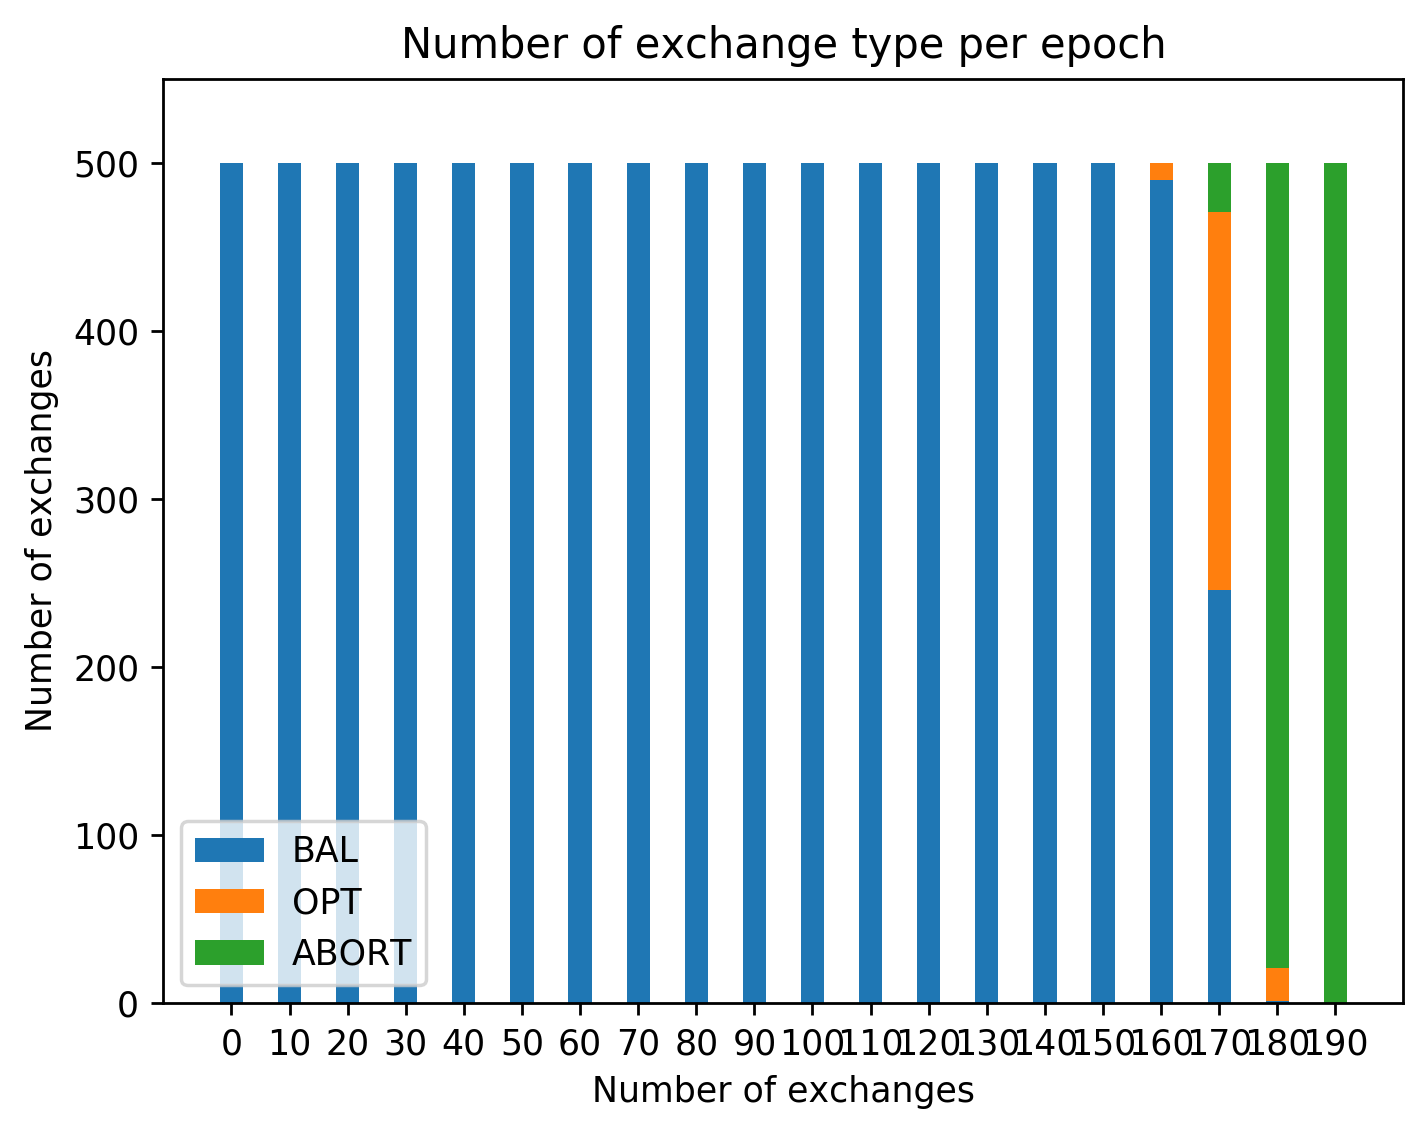
\includegraphics[width=\linewidth]{images/1/1-exchanges-type-epoch}
  	\caption{1st simulation exchange types per epoch}
  	\label{fig:sim-one-duplicates}
   \end{minipage}\hfill
   \begin{minipage}{0.49\textwidth}
     \centering
     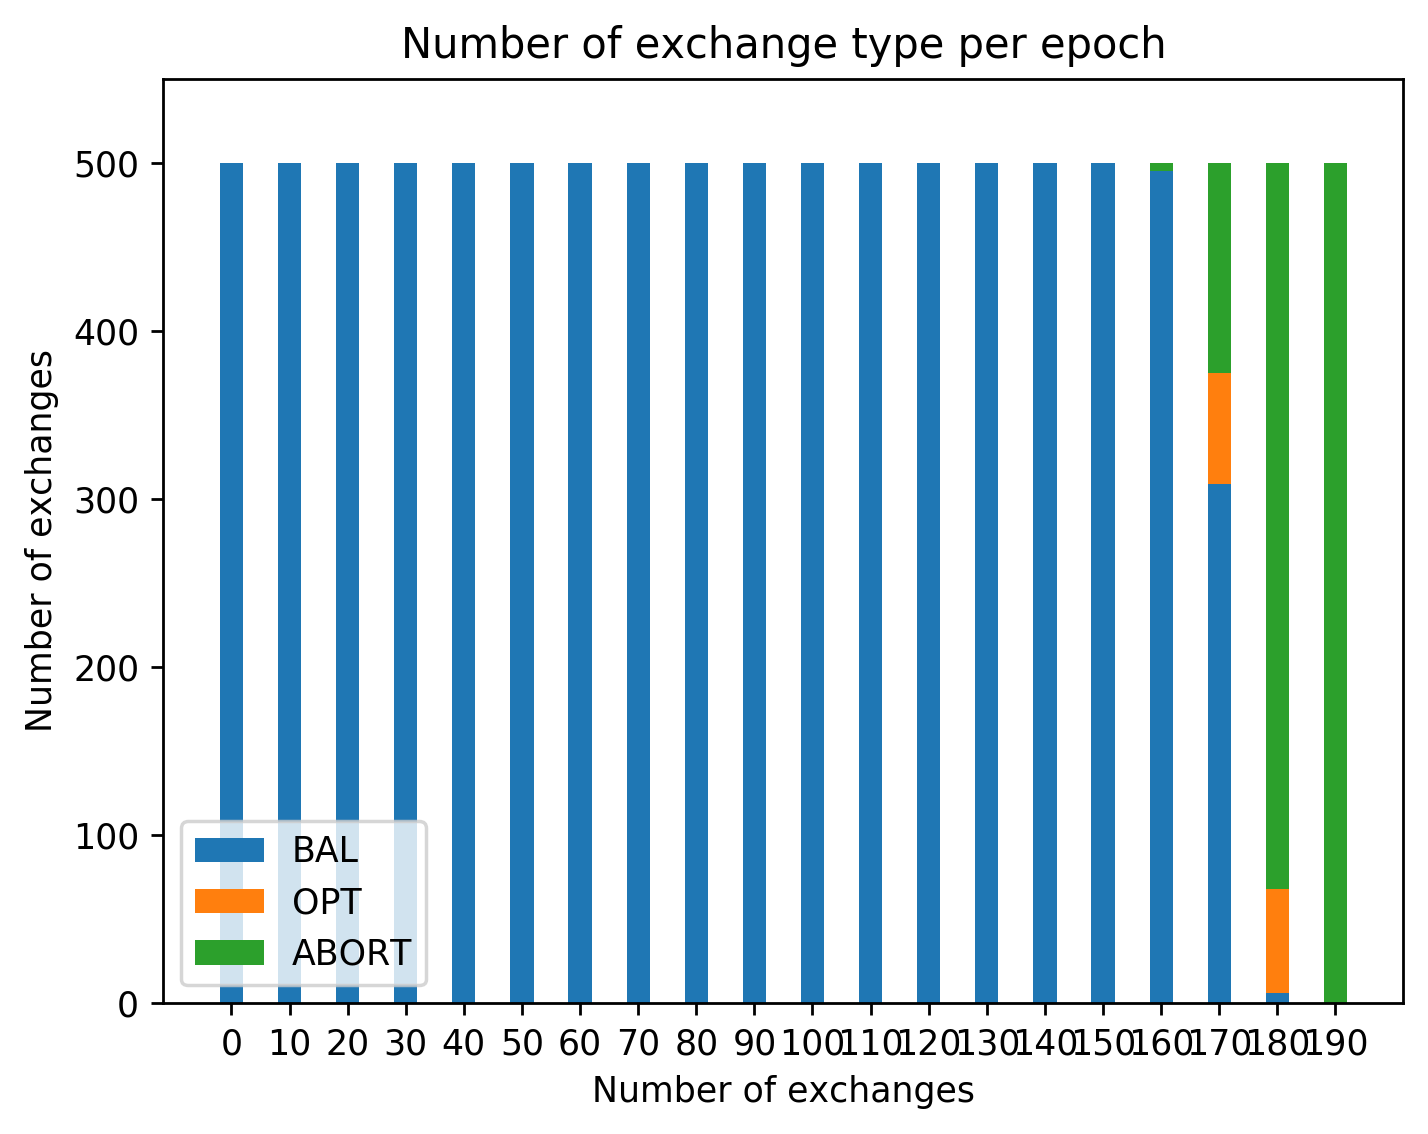
\includegraphics[width=\linewidth]{images/2/2-exchanges-type-epoch.png}
       \caption{2nd simulation exchange types per epoch }
 		\label{fig:sim-two-duplicates}
   \end{minipage}
\end{figure}

\begin{figure}[H]
  \centering
  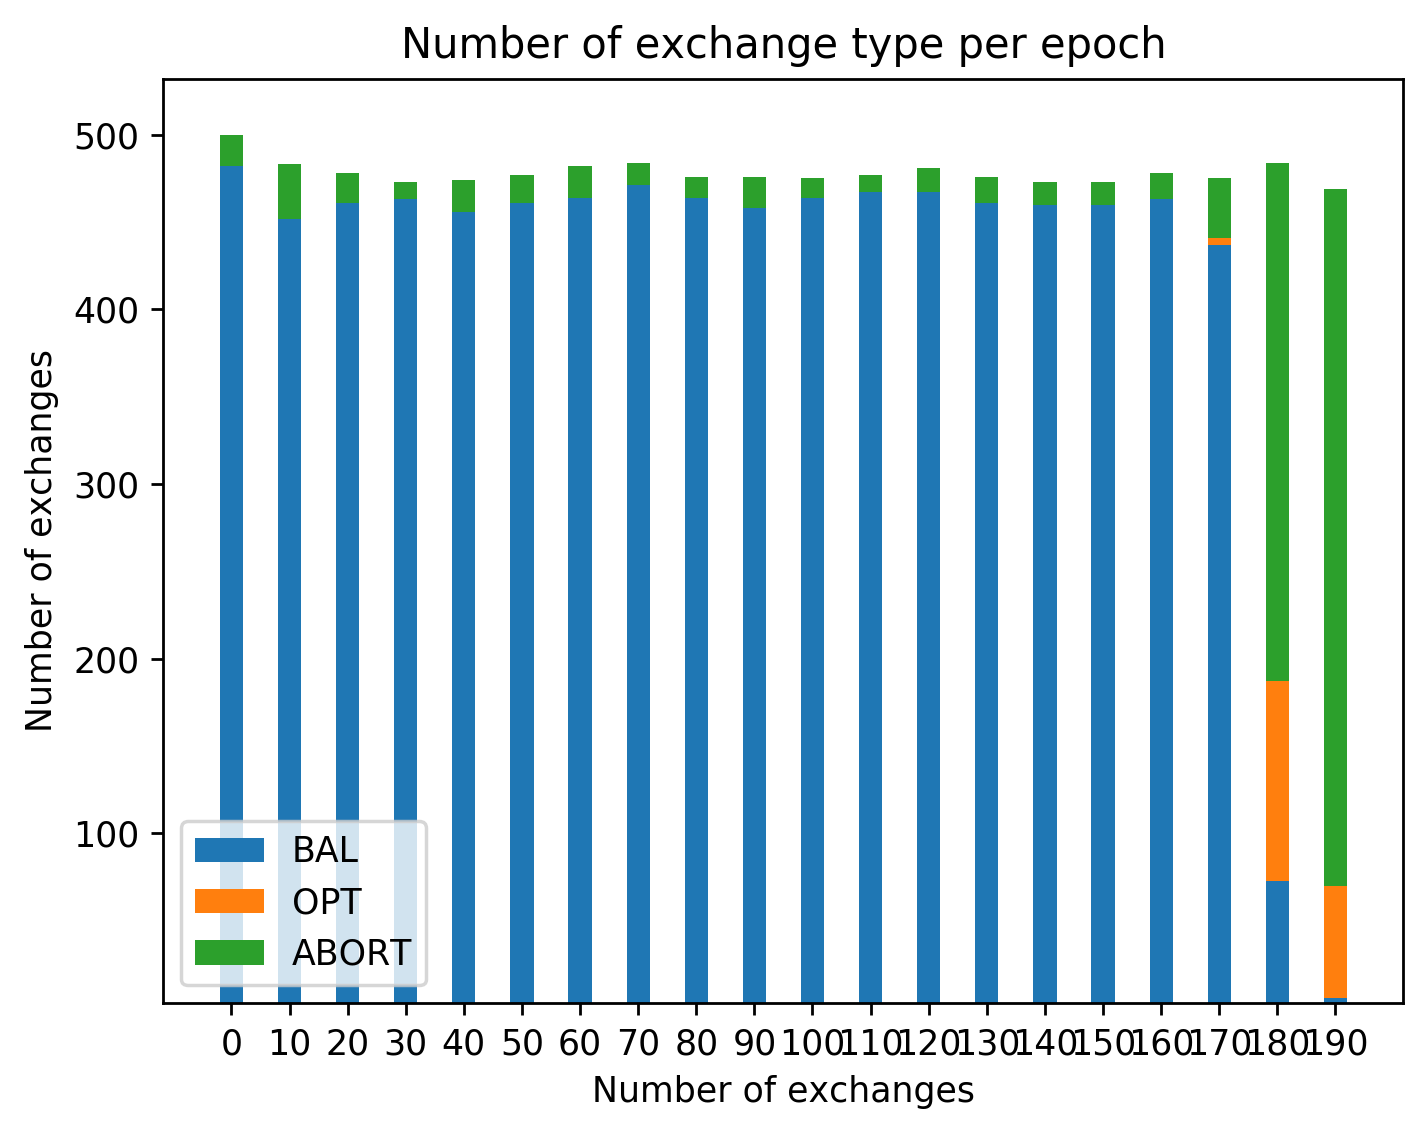
\includegraphics[width=7cm]{images/3/3-types.png}
  \caption{3rd simulation exchange types per epoch }
  \label{fig:sim-three-duplicates}
\end{figure}

It is clearly visible that the most used exchange is BAL, followed by ABORT and then OPT. Interesting is the fact that OPT exchanges are needed in the last phases of the protocol, when peers are not interested anymore in updates (as they have all of them) and only trades if they are altruistic.
In fact, the first simulation is the one containing more OPT exchanged, as everyone is altruistic. \\
Instead, the last simulation is the one with more ABORT exchange, as part of the peers act byzantine. Due to this high number of abort the network is not able to converge as fast as the two other scenarios.

\subsection{Number of exchange per epoch}
The last interesting metric is the number of non-aborted exchange done in each epoch.

\begin{figure}[!htb]
   \begin{minipage}{0.49\textwidth}
     \centering
     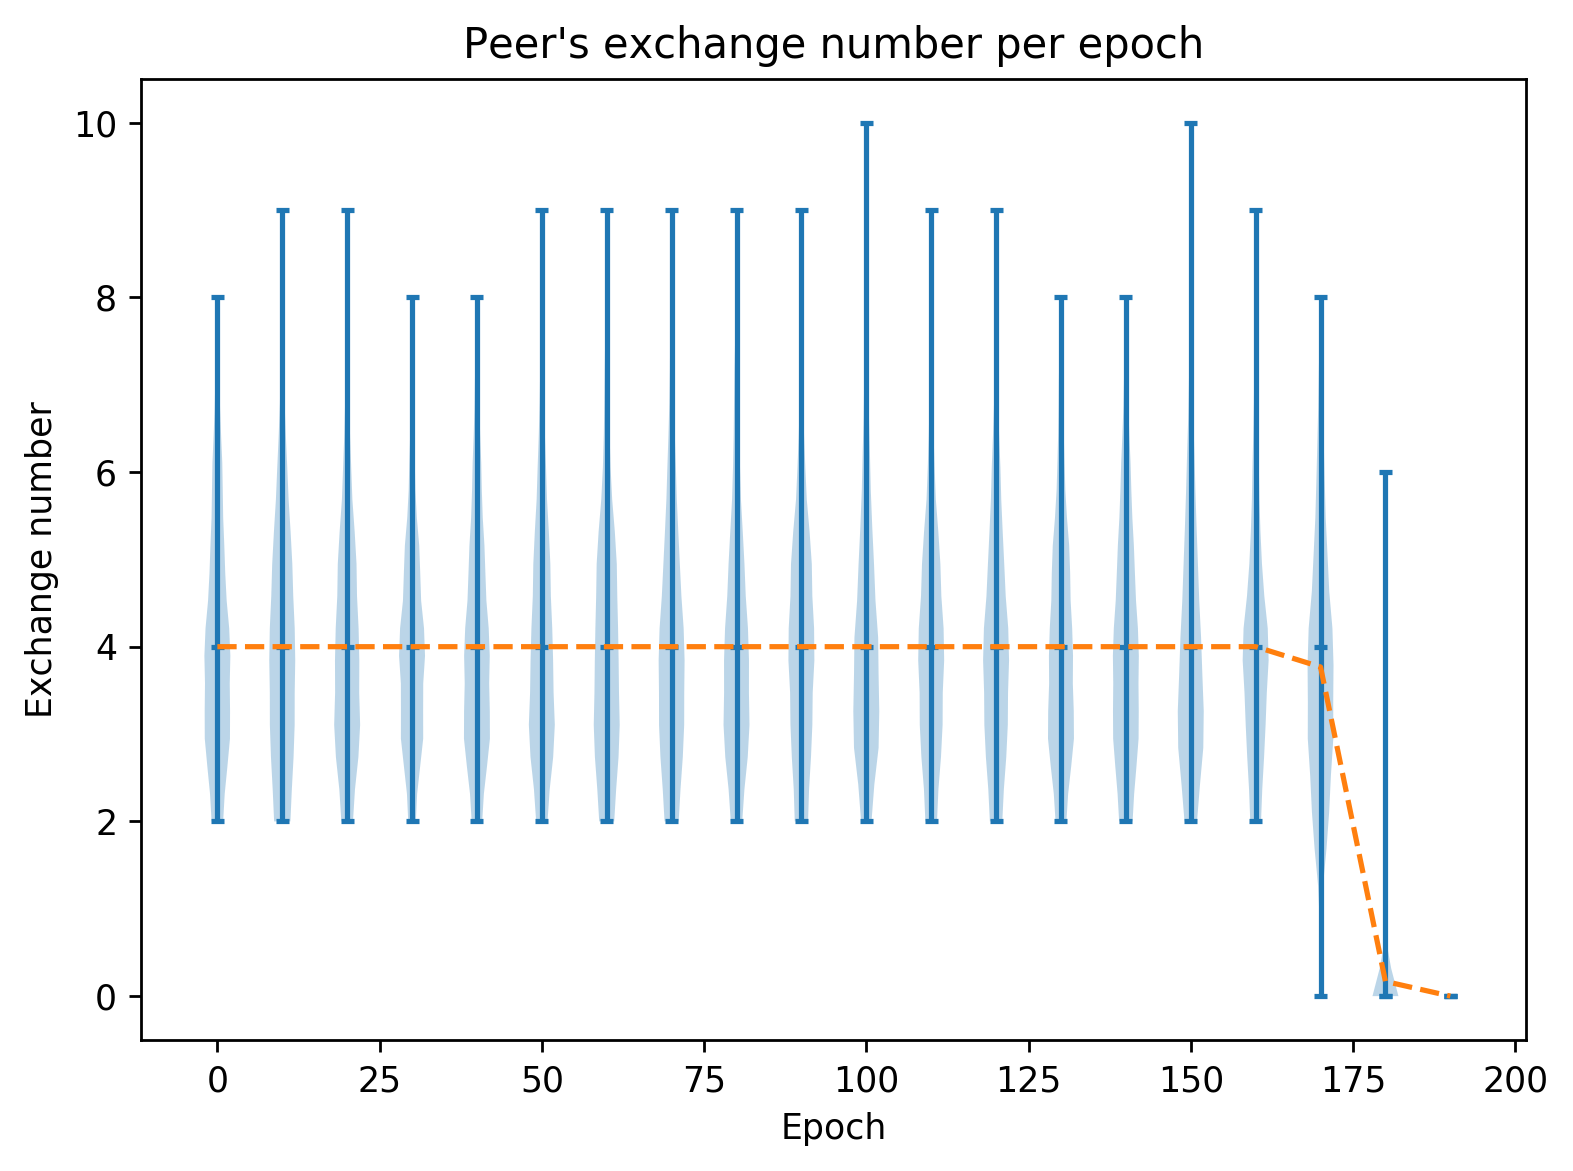
\includegraphics[width=\linewidth]{images/1/1-exchange-number-epoch.png}
  	\caption{1st simulation number of trade per peer per epoch}
  	\label{fig:sim-one-numbers}
   \end{minipage}\hfill
   \begin{minipage}{0.49\textwidth}
     \centering
     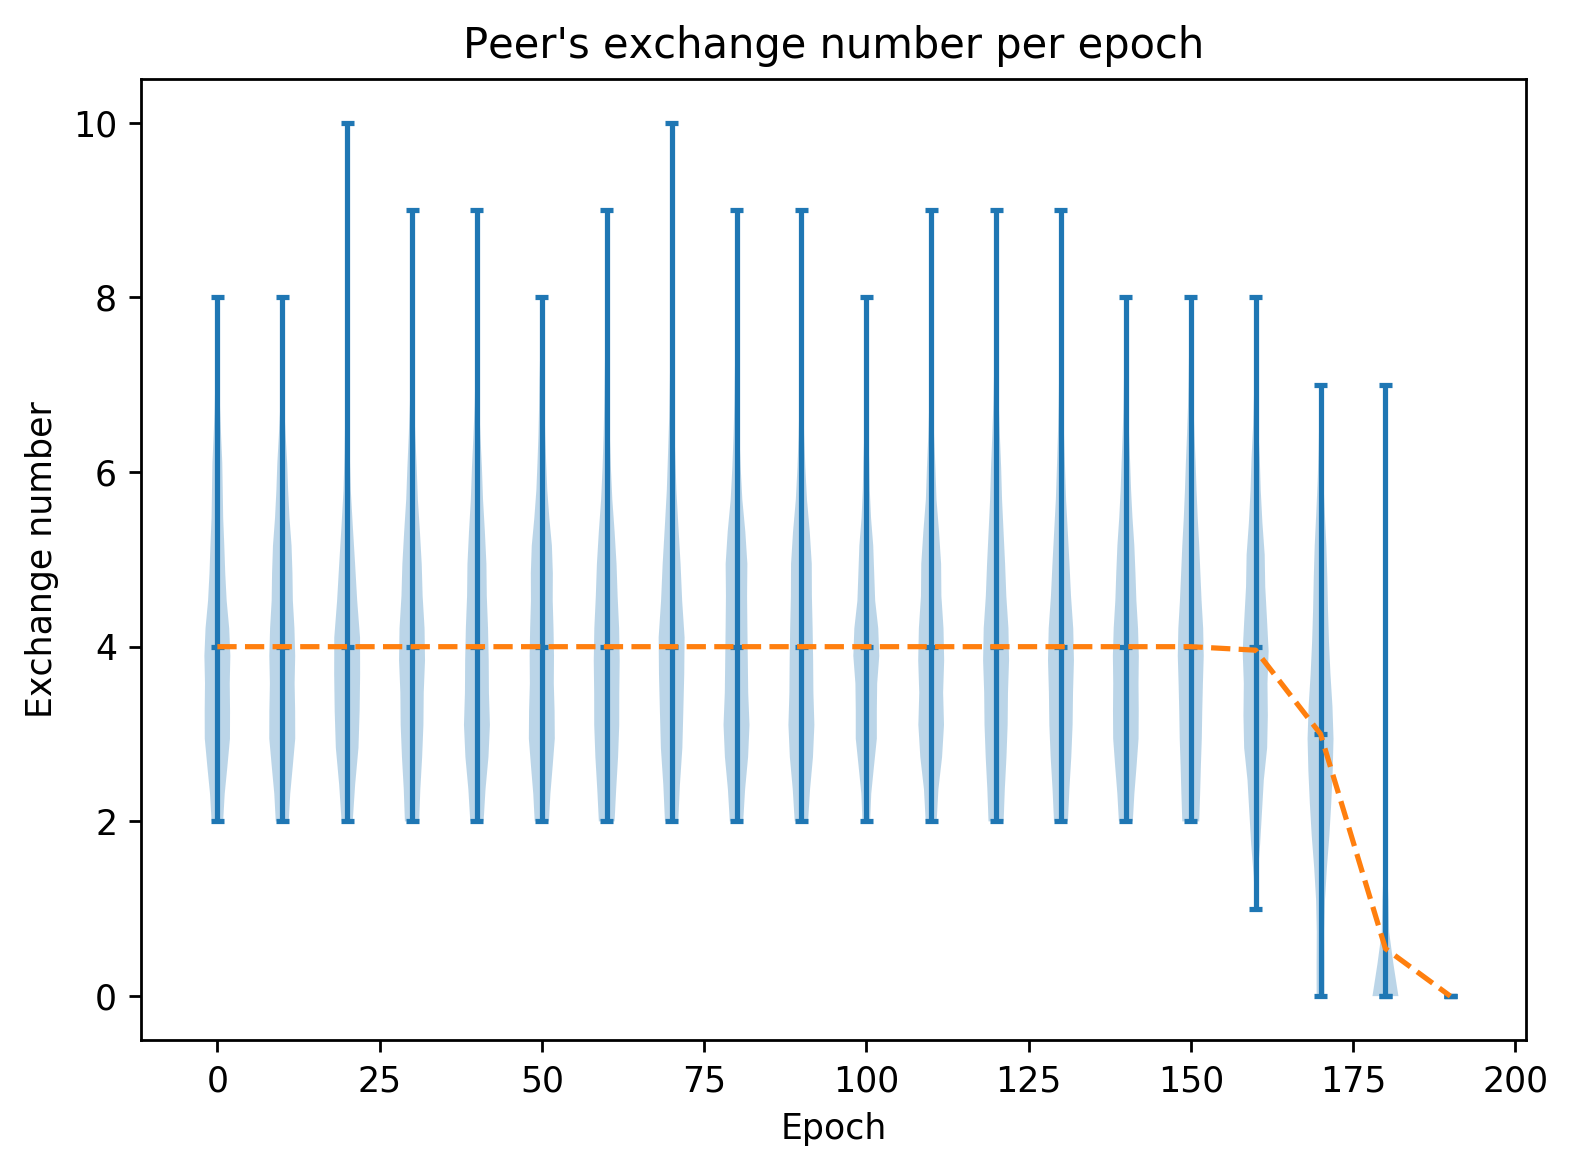
\includegraphics[width=\linewidth]{images/2/two-number-of-exchange-per-peer.png}
       \caption{2nd simulation number of trade per peer per epoch}
 		\label{fig:sim-two-numbers}
   \end{minipage}
\end{figure}

\begin{figure}[H]
  \centering
  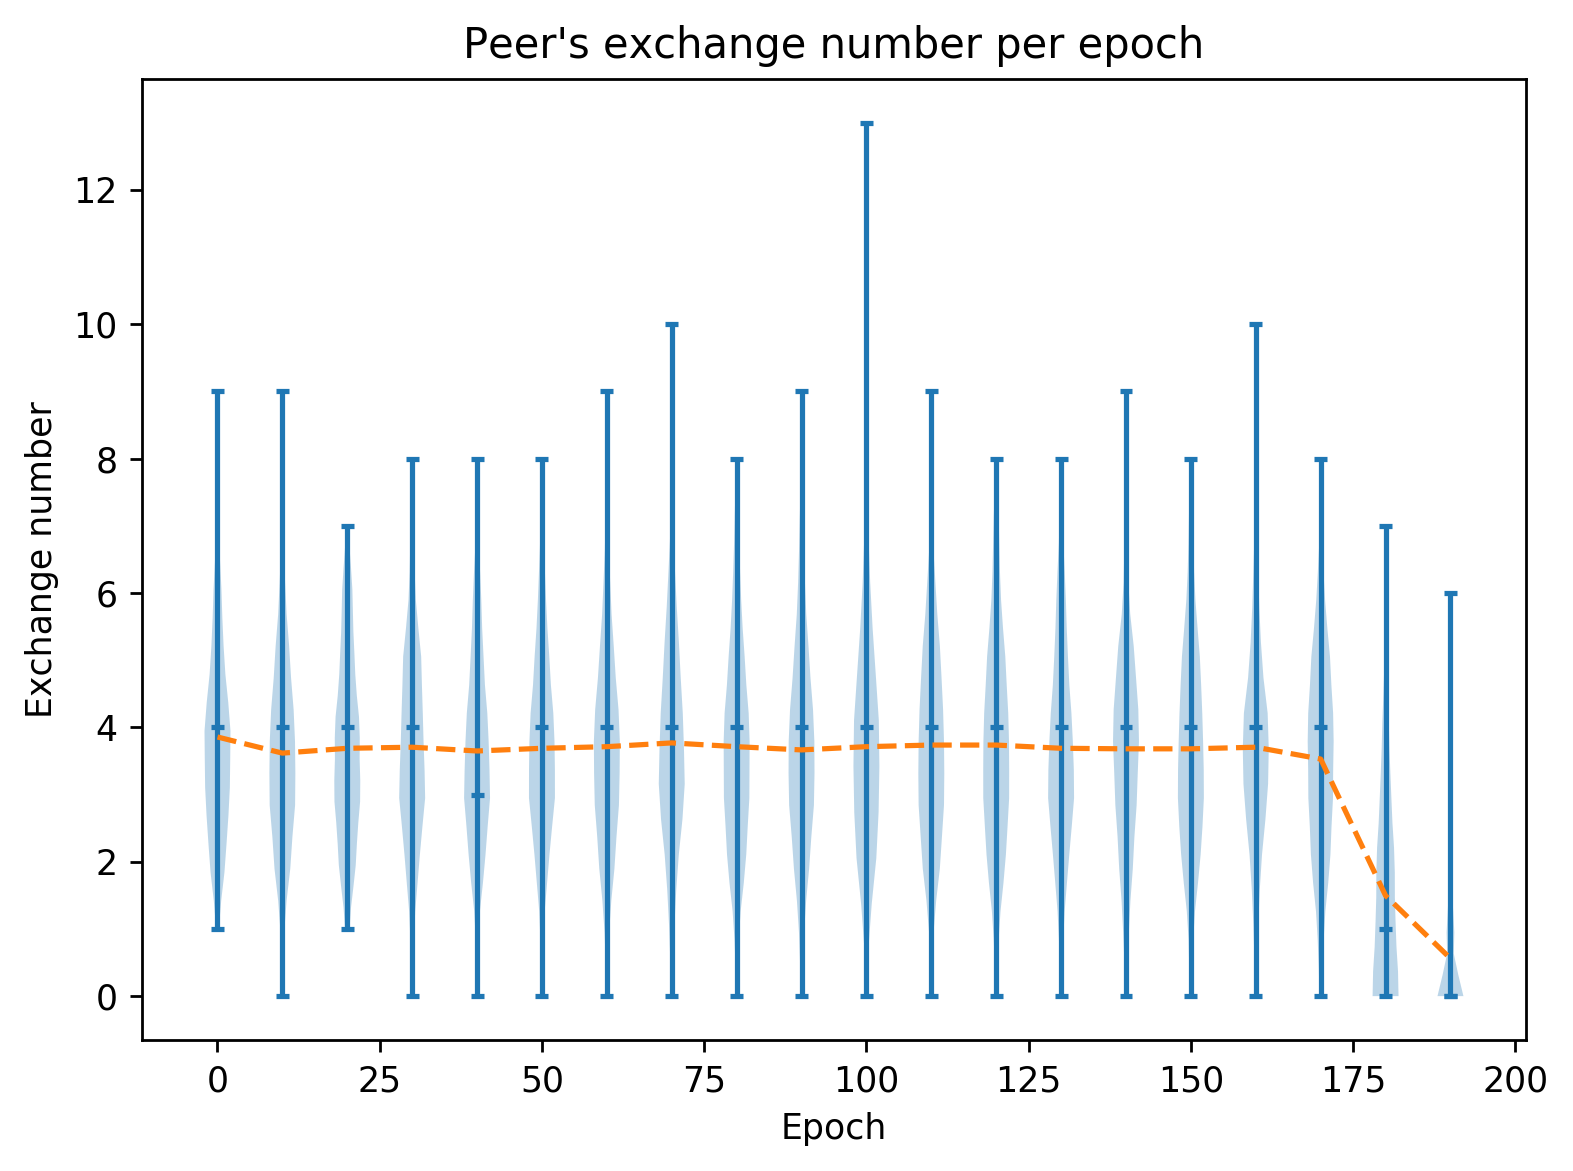
\includegraphics[width=7cm]{images/3/3-exchane-n.png}
  \caption{3rd simulation number of trade per peer per epoch}
  \label{fig:sim-three-numbers}
\end{figure}

We can instantly see that the presence of byzantine peers decrease exchange number mean in the last figure \ref{fig:sim-three-numbers}. Instead, in the the first two plots \ref{fig:sim-two-numbers} \ref{fig:sim-one-numbers}, the only difference is the steepness of the tail. This is due to the presence of rational nodes who don't want to accept OPT trades which are mostly present in the last epochs. 

\section{Insights}
\subsection{Connectivity}
The number of subscription per peer is one of the most important parameters: too low and some bootstrap node would be low connected to the network or even disconnected meaning that peers wouldn't be able to receive information from the whole network.
Instead, a too high parameters would create too many exchange, meaning a higher number of duplicates and wasted bandwidth. 

\begin{figure}[!htb]
   \begin{minipage}{0.49\textwidth}
     \centering
     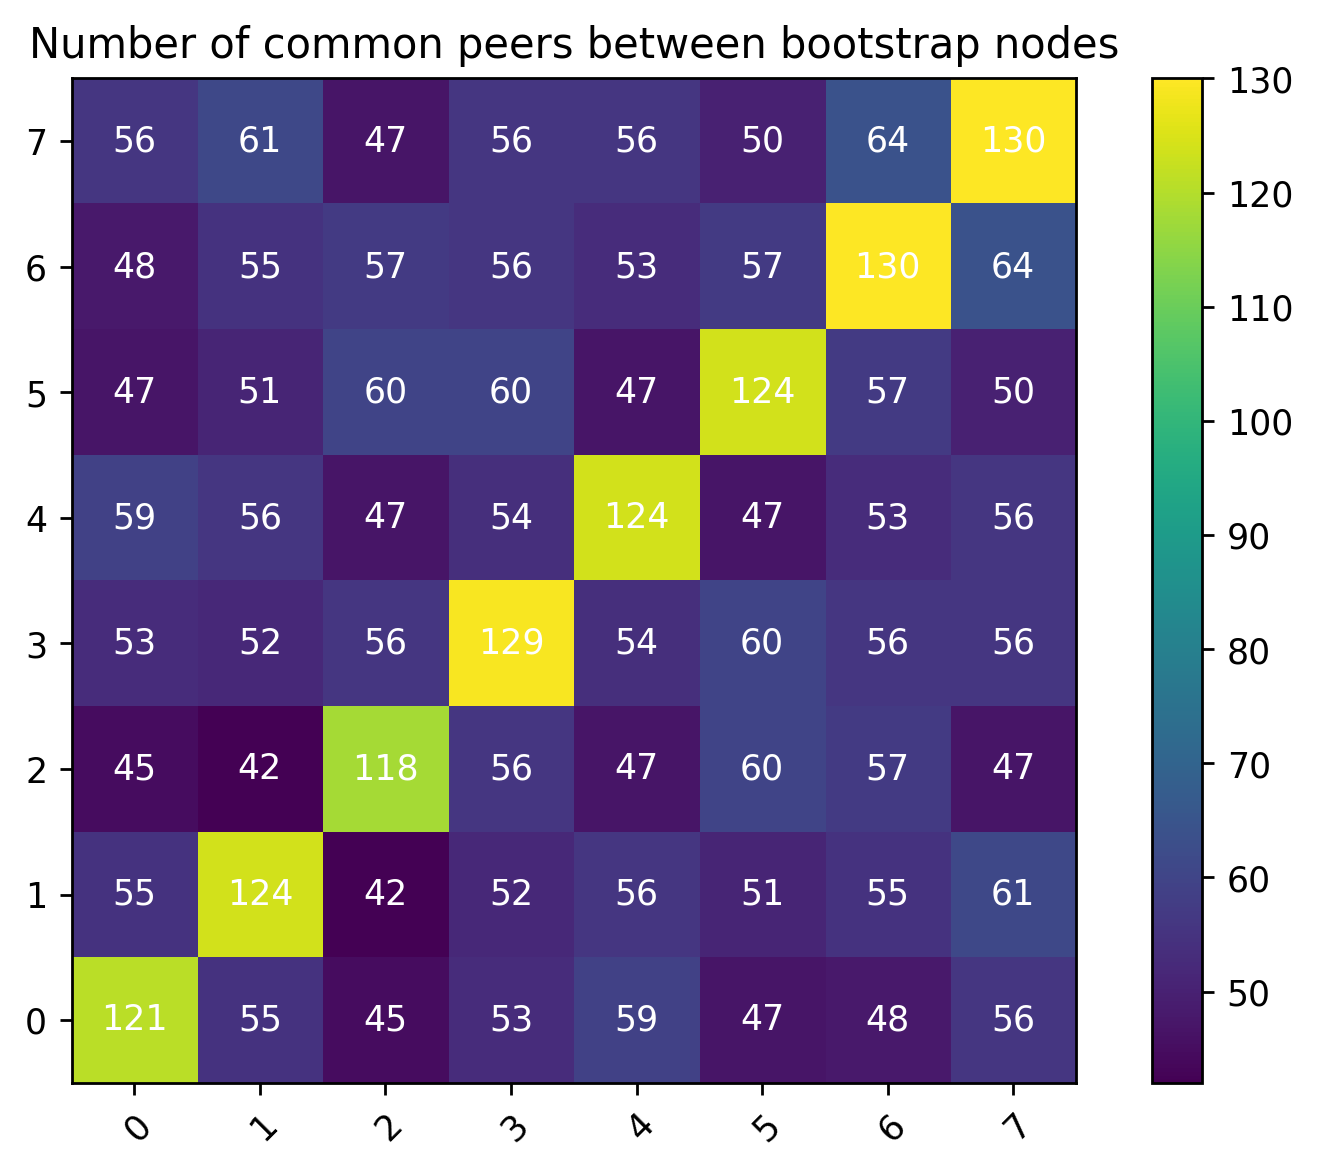
\includegraphics[width=\linewidth]{images/4/4-heatmap.png}
  	\caption{4th Simulation heatmap}
  	\label{fig:sim-one-conv}
   \end{minipage}\hfill
   \begin{minipage}{0.49\textwidth}
     \centering
     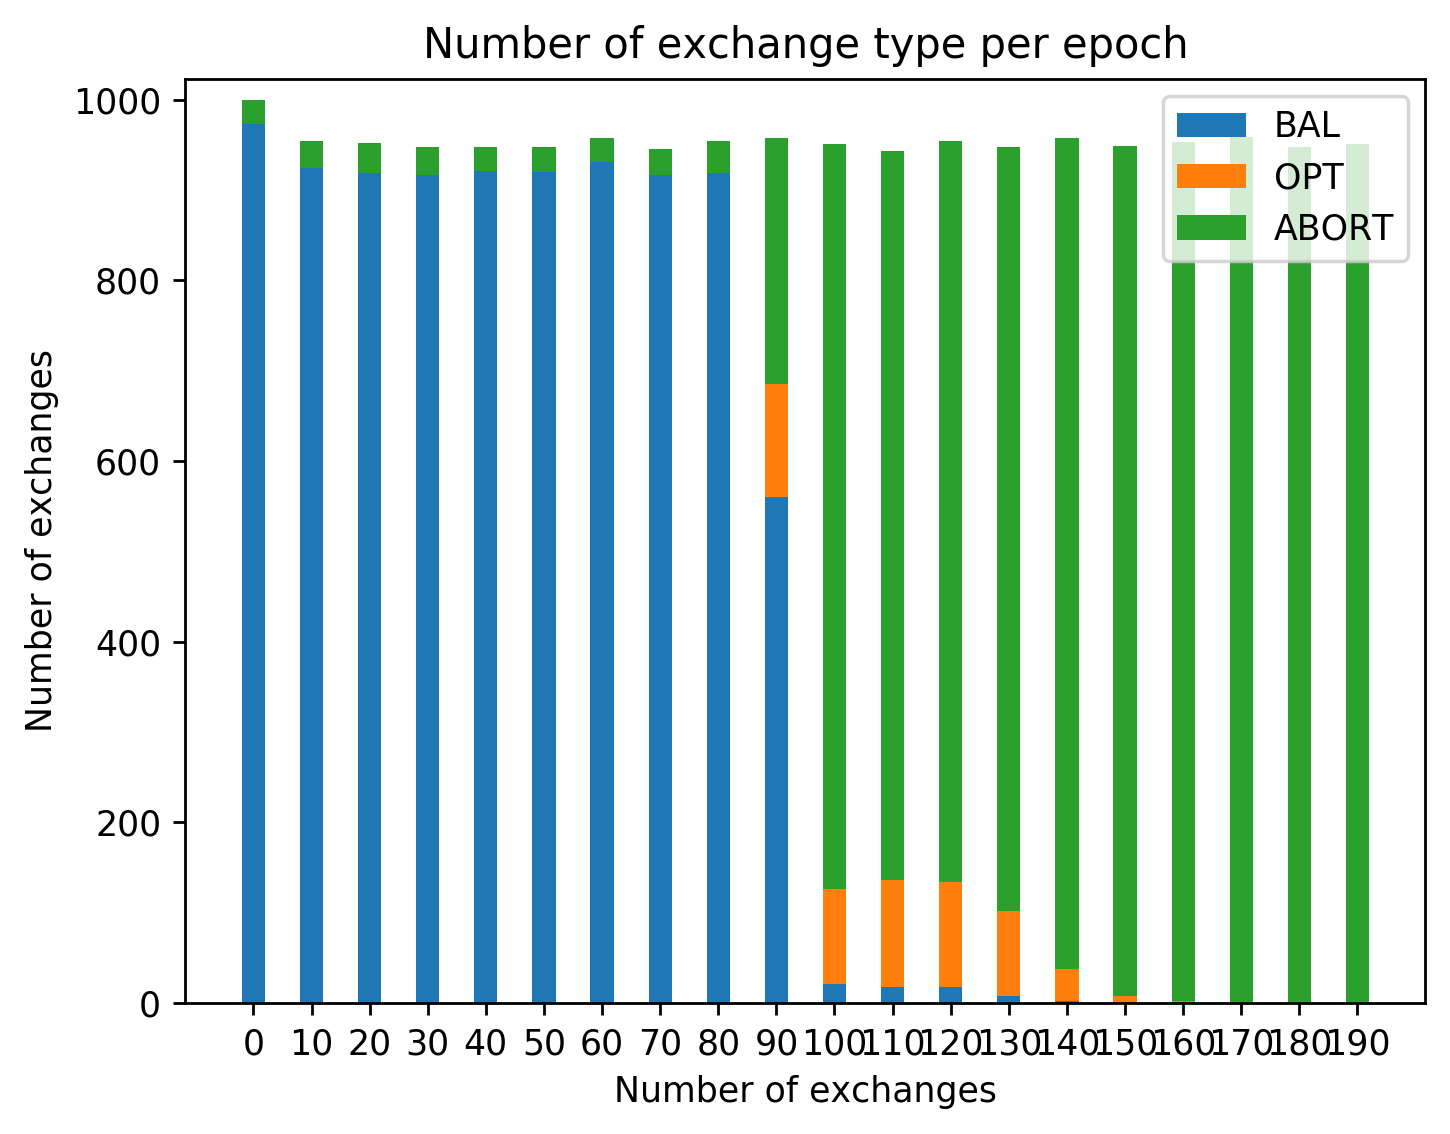
\includegraphics[width=\linewidth]{images/4/4-ex-type.png}
       \caption{4th simulation exchange types}
 		\label{fig:sim-two-conv}
   \end{minipage}
\end{figure}

\begin{figure}[!htb]
   \begin{minipage}{0.49\textwidth}
     \centering
     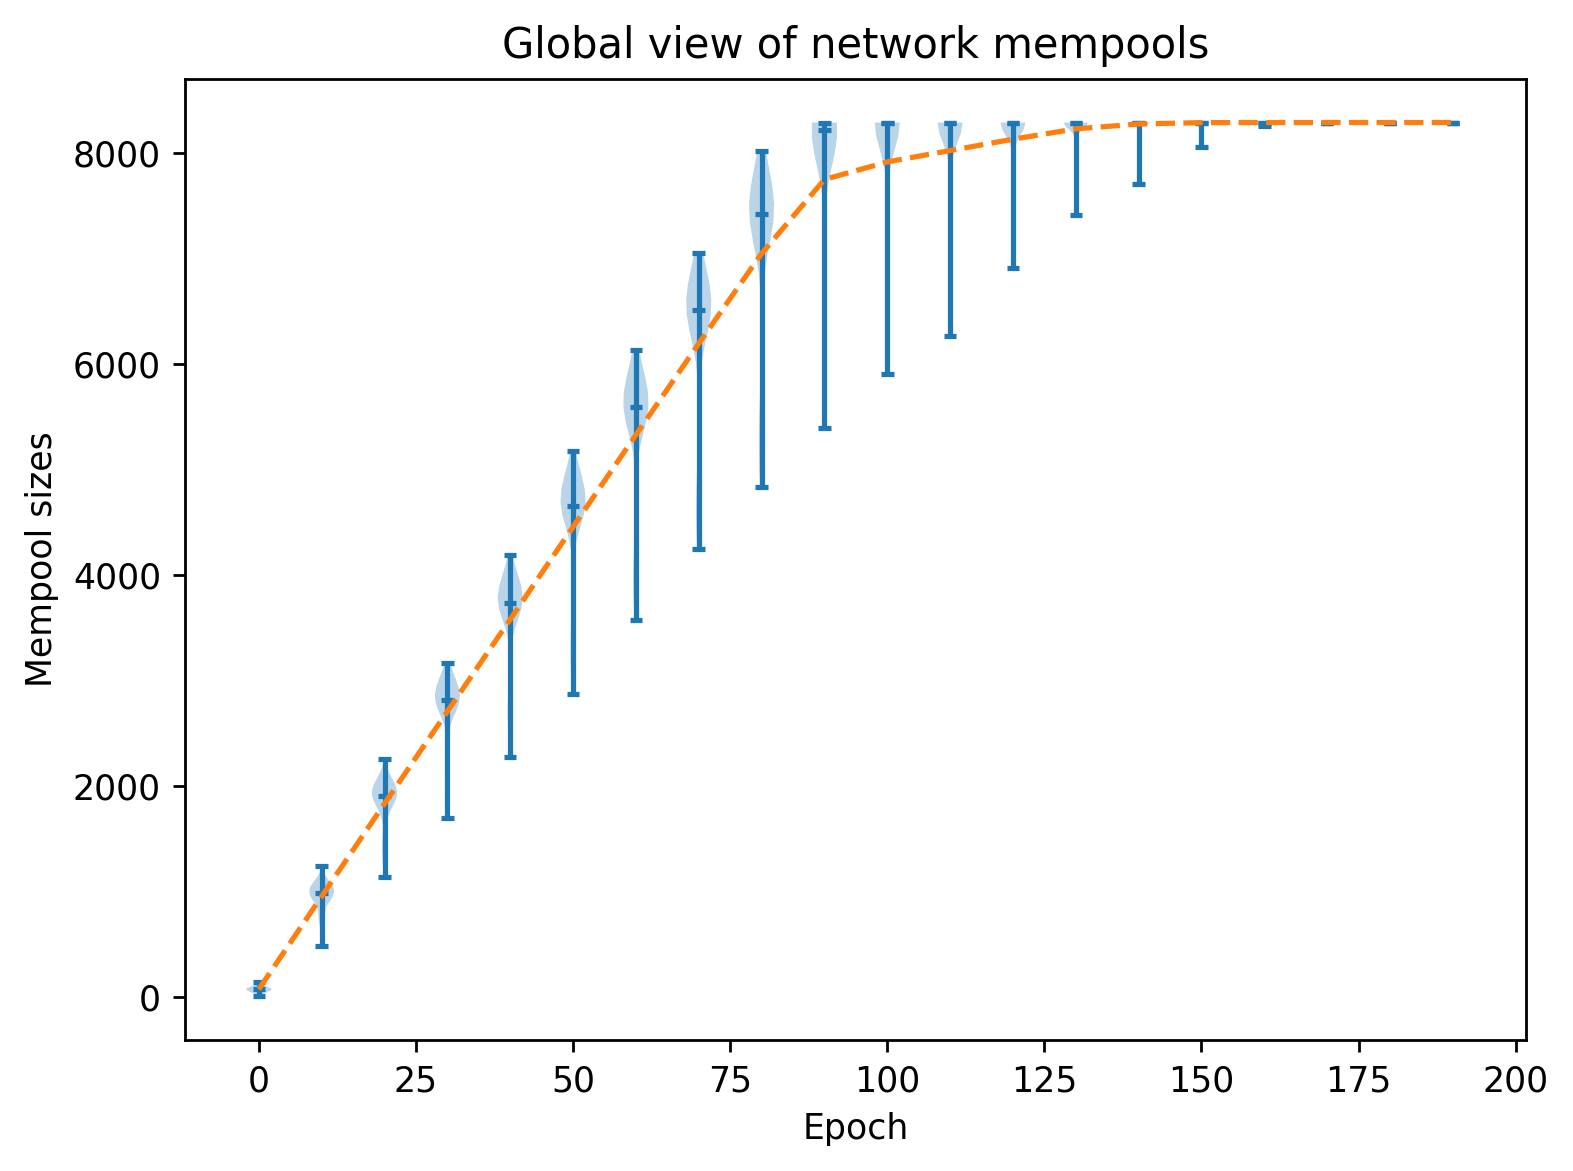
\includegraphics[width=\linewidth]{images/4/4-conv.png}
  	\caption{4th simulation convergence rate}
  	\label{fig:sim-forth-conv}
   \end{minipage}\hfill
   \begin{minipage}{0.49\textwidth}
     \centering
     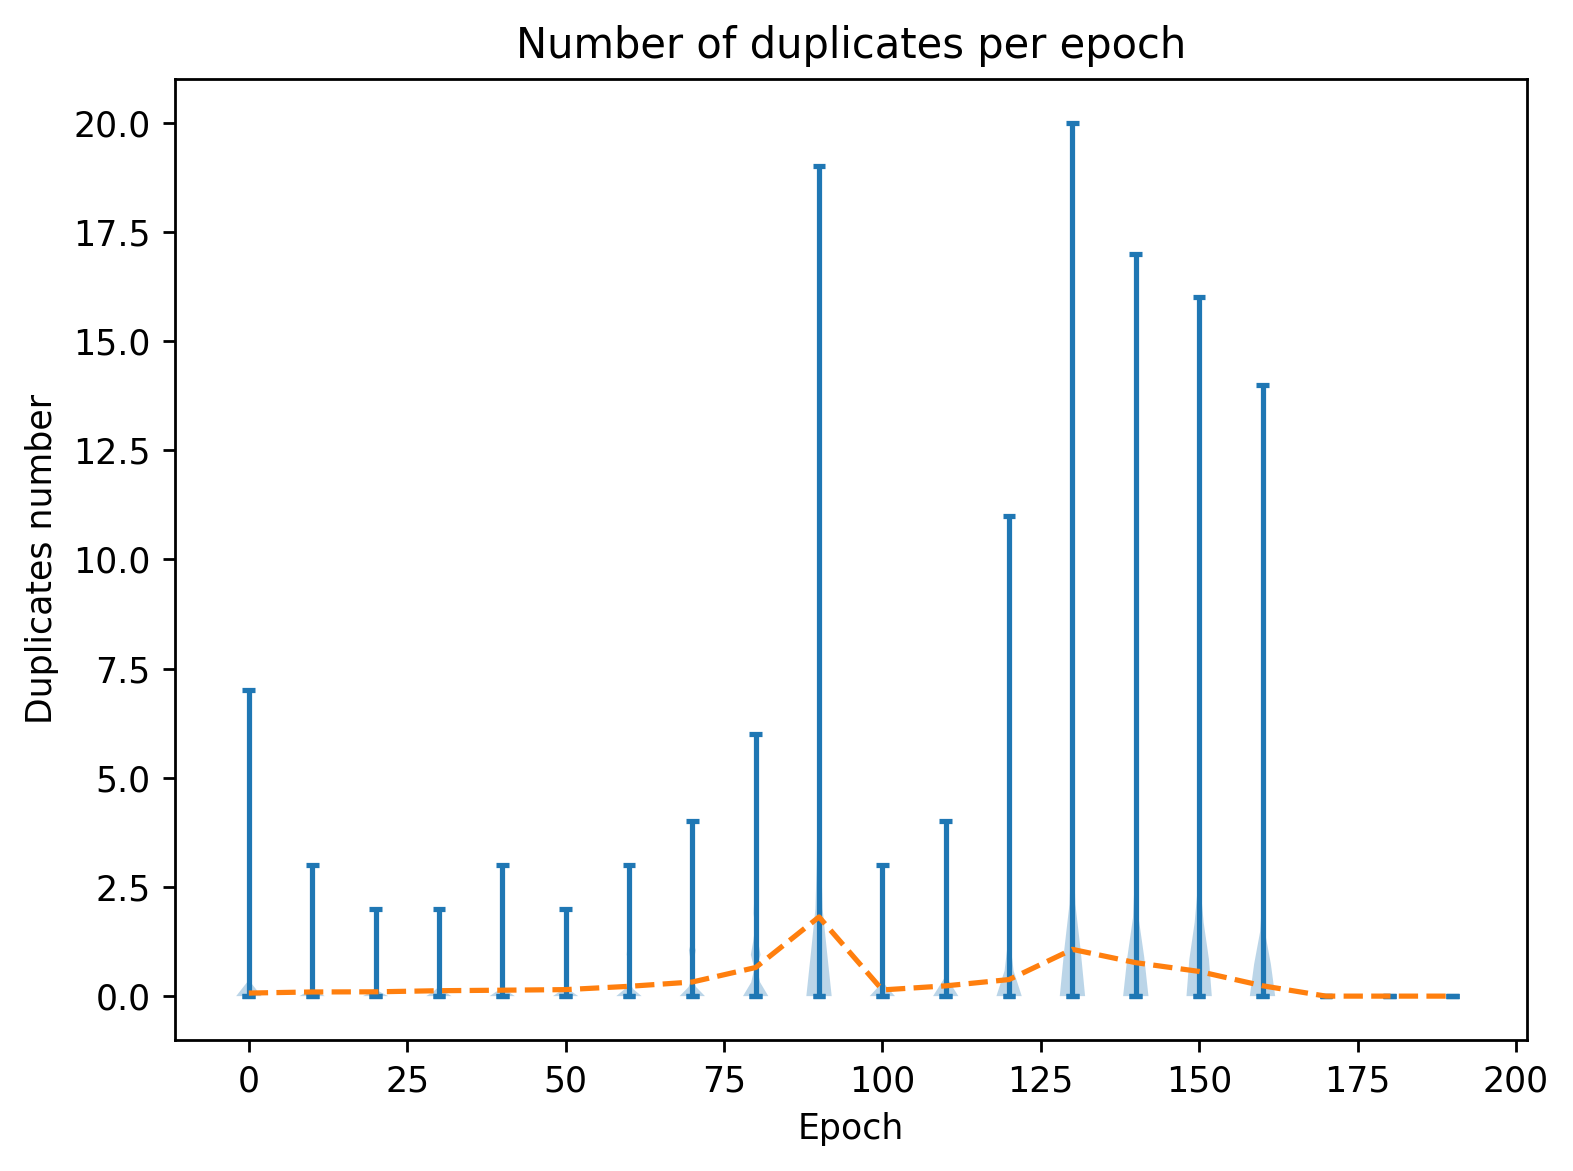
\includegraphics[width=\linewidth]{images/4/4-duplicates.png}
       \caption{4th simulation duplicates per epoch}
 		\label{fig:sim-forth-duplicates}
   \end{minipage}
\end{figure}

In order to prove this arguments we have run a simulation with the same parameters as our third, but a number of subscription of 4. \\
Due to the fact that, on average, each peer completes 2 trades per epoch per bootstrap node, with 4 bootstrap node we have a total of 8 connection per peer. This drastically increase the number of received updates meaning a faster convergence rate as shown in \ref{fig:sim-forth-conv}. It also means a higher number of duplicates \ref{fig:sim-forth-duplicates}. \\
We also want to point out that the a higher convergence rate could be archived by incresing the number of max update sharable in a BAL or OPT trade. Even if this is true, it would limit the fact that we want maximize the total number of BAL updates. Moreover, a less clustered network is more robust and reliable to synbil and eclipse attacks. 

\chapter{Conclusion}
\section{Discussion}
\section{Future works}

\chapter{Glossary}

\bibliographystyle{plainnat}
\bibliography{biblio}

\lipsum

\end{document}
